\pagebreak

% \pagestyle{empty} % Prevent numbering on the skipped page

\pagenumbering{arabic} % Set page numbering style to Arabic
\setcounter{page}{1} % Start page numbering from 2


\begin{itemize}
  \item[\textcolor{white}{$\Box$}] 
\end{itemize}


\vspace{7cm}

\begin{figure}[H]
  
\includegraphics{Images/introduction.png}
\end{figure}

\pagebreak

\pagenumbering{arabic} % Set page numbering style to Arabic
\setcounter{page}{2} % Start page numbering from 2

\section*{}
\addcontentsline{toc}{section}{INTRODUCTION}


\noindent La contraception est un enjeu primordial de santé publique, visant à améliorer la santé des femmes, des enfants et des familles ainsi que le développement socio-économique des pays, en particulier des pays en voie de développement comme le Maroc et d’autres pays Africains. Fondamentale pour la régulation des naissances, la contraception offre une multitude d’avantage cruciaux : 

\begin{tcolorbox}[colback=white, colframe=white]
  \textbf{•	Prévention des grossesses à risque : }Elle constitue une mesure de prévention essentielle pour les femmes à partir de la quarantaine, celles ayant déjà eu de nombreux enfants, les jeunes adolescentes et dans le cas de contre-indications médicales.\vspace*{1em}

  \textbf{•	Espacement des naissances : }En contribuant à l’espacement des naissances, la contraception permet de réduire le risque d’anémie chez la mère, offre plus de temps pour l’allaitement, améliorant ainsi la santé de l’enfant, et contribue à la diminution de la mortalité des nouveau-nés et des enfants.\vspace*{1em}

  \textbf{•	Prévention des grossesses non désirées : }Elle joue un rôle majeur dans la prévention des avortement liés à des grossesses non désirées, réduisant ainsi le risque pour la santé maternelle, l’infertilité et la mortalité maternelle.  \vspace*{1em}

  \textbf{•	Dépistage des infections sexuellement transmissibles :}   La contraception favorise le dépistage précoce des infections sexuellement transmissibles et d’autres maladies, contribuant ainsi à la santé reproductive globale. \vspace*{1em}

  \textbf{•	Réduction des décès maternels et infantiles : } Elle s’inscrire comme une mesure préventive cruciale pour réduire les décès maternels et infantiles. (1) \vspace*{1em}
  
  \end{tcolorbox}

\noindent Dans les années 1950, on a découvert que la progestérone bloquait l’ovulation d’où le développement de la pilule contraceptives orale combinée. C’est la méthode de contraception la plus répandue dans la plupart des pays occidentaux.(2) L’un des principaux défis de cette méthode, outre ses effets indésirables, est le manque d’observance, en particulier chez la population qui n’est pas instruite ou chez les femmes qui ne comprennent pas les conséquences d’un manque d’observance. Les études ont montré qu’au moins une fois par mois, une femme sur cinq oublie de prendre sa pilule contraceptive.(3) \vspace*{1em}
 
\noindent Nous disposons aujourd’hui de nombreuses méthodes de contraception qui peuvent être classées en deux catégories principales : les méthodes hormonales qui comprennent les contraceptifs oraux, les contraceptifs injectables, les implants sous-cutanés, les dispositifs intra-utérins hormonaux, etc., et les méthodes de contraception non hormonales, qui comprennent les méthodes naturelles de contraception, les méthodes chirurgicales et le stérilet en cuivre. Parmi ces méthodes, certaines peuvent résoudre le problème d’observance et présentent d’autres avantages. \vspace*{1em}

\noindent Dans cette étude  nous nous focaliserons plus particulièrement sur la contraception injectable. 
Elle fait partie du programme Marocain de planification familiale.(4) Il s’agit d’une méthode contraceptive très efficace avec un taux d’échec très faible si les protocoles sont dûment respectés. Elle est venue combler le problème d’oubli de la pilule journalière  mais est-elle acceptée ? \vspace*{1em}

\noindent Cette étude évalue l’acceptabilité de la contraception injectable par les femmes dans les centres de santé publique de quatre villes du Maroc (Rabat, Salé, Kénitra et Témara) à travers le regard des professionnels de santé qui jouent un rôle particulier dans sa mise en œuvre.\vspace*{1em}

\pagebreak

\begin{itemize}
  \item[\textcolor{white}{$\Box$}] 
\end{itemize}


\vspace{7cm}

\begin{figure}[H]
  
\includegraphics{Images/partie_theorique.png}
\end{figure}


\section*{}
\addcontentsline{toc}{section}{PARTIE I: THEORIQUE}
% \nocite{munoz2011contraception}
% \nocite{lhagadang2021contraception}
% \nocite{nejm_hormonal_contraception}
% \nocite{standards_maroc}
% \nocite{vincent-rohfritsch2012nouveautes}
% \nocite{naudon2022tour}
% \nocite{localisationuterus}
% \nocite{martin2004atlas}
% \nocite{tachdjian2016appareil}
% \nocite{hoare2024anatomy}
% \nocite{lhagadang2021contraception}
% \nocite{*}

\pagebreak


\section{Généralités sur la contraception}
\subsection{Définition: }
La contraception est définie comme l’ensemble des méthodes qui permettent d’éviter les grossesses non désirées et d’espacer les naissances.(5) \vspace*{1em}

\subsection{Rappel sur l’appareil reproducteur féminin: }
L’appareil reproducteur féminin est composé des organes génitaux externes et internes. (6)\\

\noindent Les organes génitaux externes englobent les structures visibles à l'extérieur du bassin, comprenant les grandes et petites lèvres, le vestibule, les glandes de Bartholin, le clitoris, le périnée, les glandes de Skene, le pubis, le méat urétral et la zone péri-urétrale. (6)\\

\noindent La vulve, qui se trouve entre les petites lèvres, correspond au vestibule du vagin. Les glandes de Bartholin sont situées de chaque côté du vestibule vaginal. Les petites lèvres sont des plis de muqueuse qui contiennent de nombreuses glandes sébacées et sudoripares, ainsi qu'une innervation sensitive importante. Quant aux grandes lèvres, ce sont des renflements de la peau qui sont particulièrement riches en follicules pileux, glandes sébacées et sudoripares à leur surface externe. Le clitoris, quant à lui, est un organe érectile. (7) 

\pagebreak


\begin{figure}[H]
  \centering
  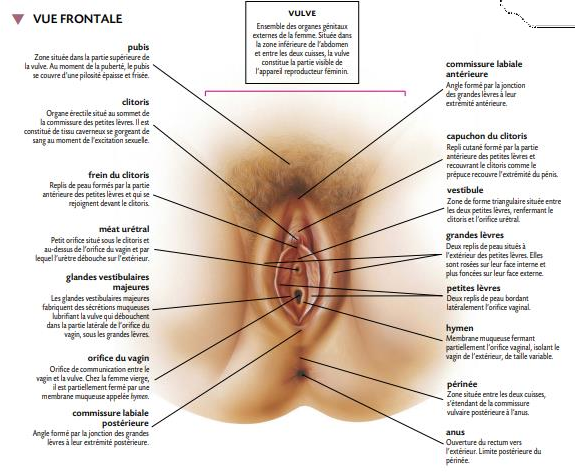
\includegraphics{Images/fig_1.png}
  \caption{Schéma montrant une vue frontale de la vulve (8)}
\end{figure}

\vspace*{1em}


\noindent Quant aux organes génitaux internes, ils résident à l'intérieur du bassin et incluent les ovaires, les trompes de Fallope, l'utérus, le col de l'utérus et le vagin. Ces organes jouent un rôle crucial dans les processus de reproduction et de régulation hormonale chez la femme. (6) \vspace*{1em}

\noindent Les ovaires se trouvent dans le pelvis et ont pour rôle principal la production de stéroïdes sexuels et la formation des ovules. Leur fonction varie selon les différentes phases du cycle menstruel. Les trompes utérines assurent le transport des gamètes et des embryons, et c'est généralement à ce niveau que la fécondation se produit. L'utérus est un organe pelvien positionné entre la vessie en avant et le rectum en arrière. Il comprend une partie dilatée appelée corps utérin, dont la partie supérieure forme le fond utérin en continuant avec le col de l'utérus, qui s'ouvre dans le vagin. Le col utérin se compose de deux parties, l'endocol et l'exocol. L'endocol contient des glandes qui sécrètent la glaire cervicale, dont sa sécrétion varie également selon les différentes phases du cycle menstruel. Le vagin, quant à lui, est un conduit musculo-membraneux constitué de trois couches : une muqueuse, une tunique et un adventice. La muqueuse vaginale subit des changements cellulaires au cours du cycle menstruel. (7) \vspace*{1em}

\begin{figure}[H]
  \centering
  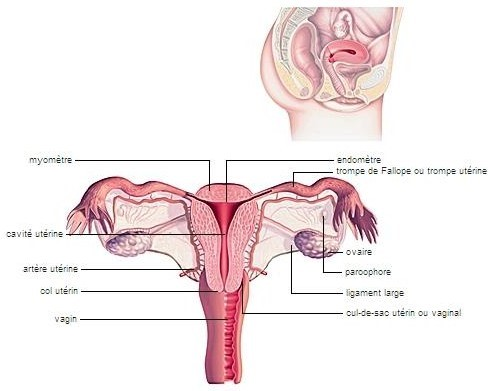
\includegraphics{Images/fig_2.jpg}
  \caption{Appareil reproducteur féminin (9)}
\end{figure}

\subsection{Rappel sur la physiologie du cycle menstruel : }

La compréhension du mécanisme d’action des différentes méthodes contraceptives nécessite une bonne connaissance de la physiologie du cycle menstruel. En effet, ce processus complexe est orchestré par le système hormonal débutant avec la libération de la gonadolibérine par l’hypothalamus. Cette hormone stimule ensuite l’hypophyse déclenchant la production des hormones folliculostimulante (FSH) et lutéinisante (LH). Ces hormones jouent un rôle crucial en influençant les ovaires à libérer des hormones sexuelles, notamment la progestérone et les œstrogènes. Ces dernières régulent divers aspects du cycle menstruel et sont essentielles à la maturation des ovules.(10) 

\begin{figure}[H]
  \centering
  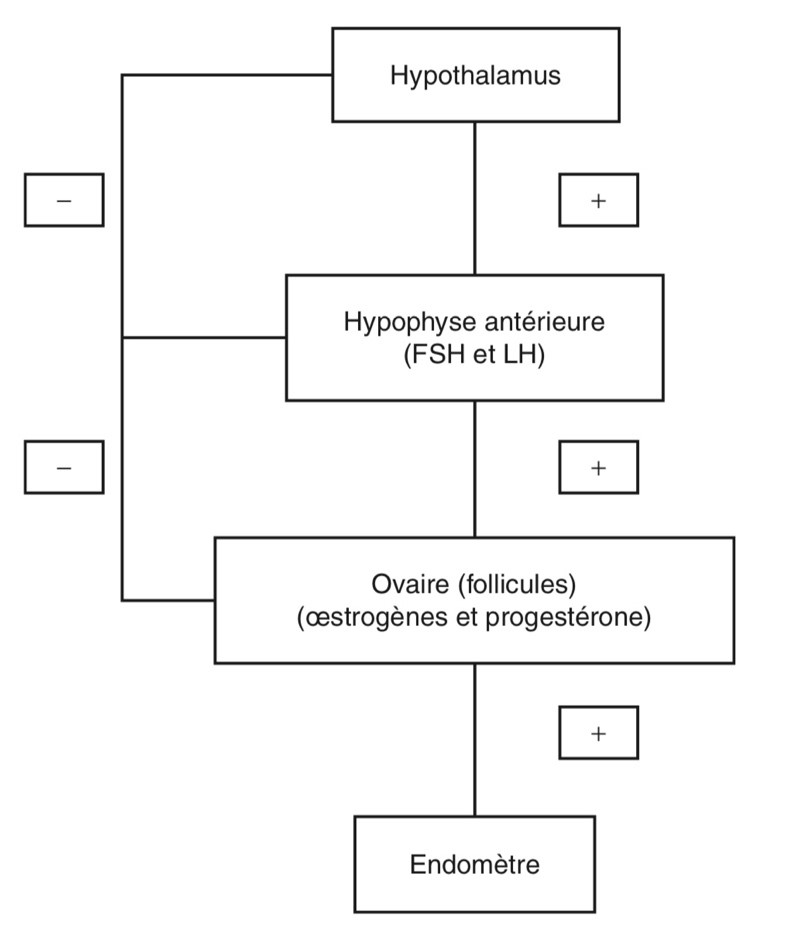
\includegraphics{Images/fig_3.jpg}
  \caption{Rétroaction biologique des hormones féminines (11)}
\end{figure}


Un cycle menstruel s'étend généralement sur une période de 28 à 32 jours, avec le premier jour marquant le début de la menstruation. (12) Ce processus naturel peut être subdivisé en quatre phases distinctes, chacune jouant un rôle spécifique dans le fonctionnement du cycle reproducteur féminin.


\hspace{1em}\textbf{•	La phase menstruelle:} \vspace{.5em}

\noindent Durant cette phase, le corps jaune, en cours de maturation, entraîne une diminution des niveaux d'hormones sexuelles, déclenchant ainsi le processus de desquamation de l'endomètre et le début des règles. Cette phase est généralement d'une durée d'environ cinq jours. 
  
\begin{figure}[H]
  \centering
  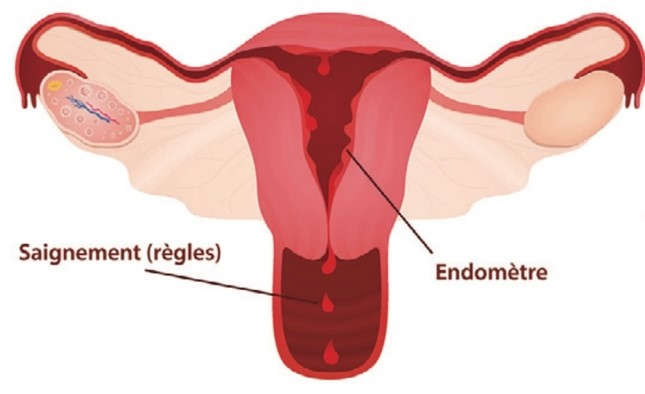
\includegraphics{Images/fig_4.jpg}
  \caption{La phase menstruelle }
\end{figure}


\hspace{1em}\textbf{•	La phase folliculaire: } \vspace{.5em}

\noindent Cette phase précède l’ovulation. La FSH stimule le développement de plusieurs follicules ovariens, cependant, un seul follicule atteint sa pleine maturité. Ce follicule contient les ovocytes qui seront ultérieurement libérés lors du processus d’ovulation.

\begin{figure}[H]
  \centering
  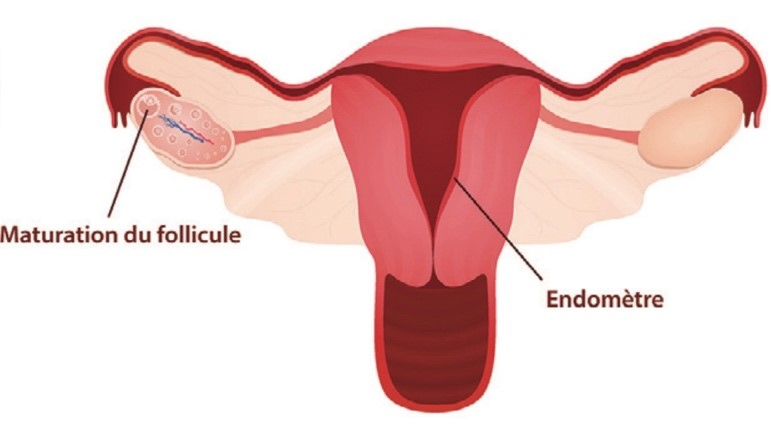
\includegraphics{Images/fig_5}
  \caption{La phase folliculaire }
\end{figure}

\hspace{1em}\textbf{•	La phase ovulatoire:  } \vspace{.5em}

\noindent Cette phase se produit généralement vers le quatorzième jour du cycle menstruel. À ce moment, la concentration élevée de l'hormone lutéinisante (LH) stimule la libération des ovocytes par le follicule ovarien mature.

\begin{figure}[H]
  \centering
  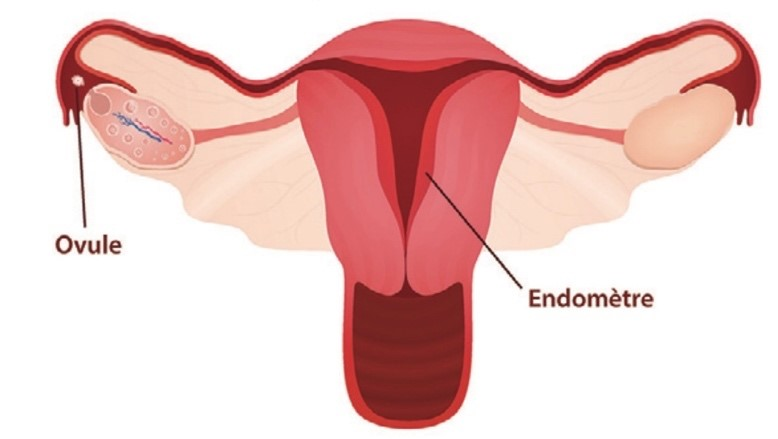
\includegraphics{Images/fig_6.jpg}
  \caption{La phase ovulatoire}
\end{figure}

\hspace{1em}\textbf{•	La phase lutéale:} \vspace{.5em}

\noindent Après l’ovulation, les niveaux de FSH et LH diminuent et le follicule rompu se transforme en corps jaune qui sécrète la progestérone et des œstrogènes. Ces hormones préparent l’endomètre à l’implantation. Si la fécondation n’a pas lieu, le corps jaune dégénère, ce qui entraîne une diminution des hormones sexuelles. Cette dégénérescence marque la fin de la phase lutéale et prépare l’organisme à l’amorce du cycle menstruel suivant.   

\begin{figure}[H]
  \centering
  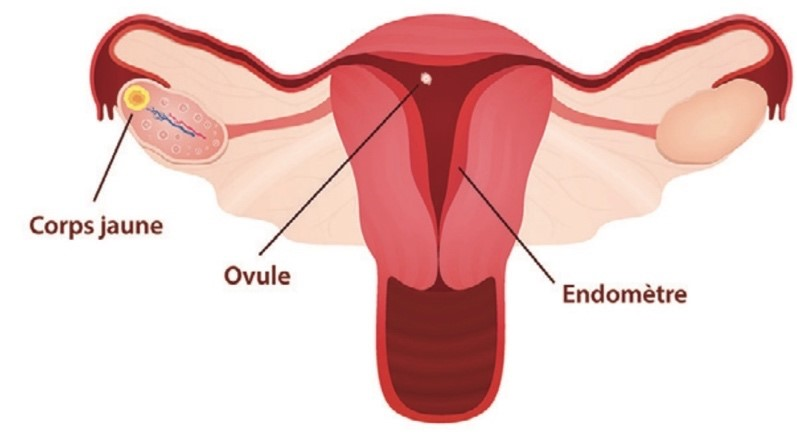
\includegraphics{Images/fig_7.jpg}
  \caption{La phase lutéale (10)}
\end{figure}

\vspace{1em}

\noindent Cette cascade complexe d'événements hormonaux constitue la base sur laquelle les méthodes contraceptives agissent. En comprenant ces mécanismes, il devient possible d'apprécier comment chaque méthode vise à perturber ou moduler ces processus, offrant ainsi une protection efficace contre les grossesse non désirées.

\begin{figure}[H]
  \centering
  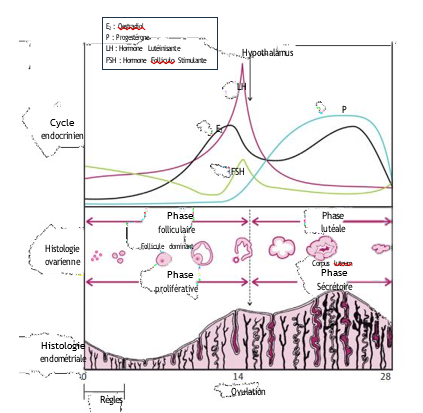
\includegraphics[scale=1.5]{Images/fig_8.jpg.png}
  \caption{Diagramme du cycle menstruel normal (13)}
\end{figure}

\subsection{Histoire de la contraception}
La pratique de la contraception remonte à des siècles, et au fil du temps, différentes méthodes ont émergé pour réguler la procréation. Certaines de ces approches historiques ont perduré jusqu'à nos jours. Voici un aperçu de quelques-unes de ces méthodes:\vspace*{1em}


\begin{itemize}[label={$\bullet$}, align=right]
  \item \textbf{La méthode du retrait:} Remontant à l'Antiquité, cette méthode consiste en l'interruption des rapports sexuels avant l'éjaculation. Bien qu'ancienne, elle est encore employée de nos jours malgré ses limitations \vspace*{0.5em}

  \item \textbf{La méthode du rythme:} Une approche basée sur le calendrier, cette méthode ancienne a évolué au fil des années. Elle repose sur la compréhension du cycle menstruel et demeure une option utilisée actuellement. \vspace*{0.5em}

  \item \textbf{La méthode Billings: }Cette méthode date des années 1960 et repose sur l'observation des sécrétions cervicales pour déterminer la période fertile de la femme. Elle est encore employée de nos jours. \vspace*{0.5em}

  \item \textbf{Les capes cervicales et les diaphragmes: }Ces dispositifs, remontant à une époque ancienne, sont toujours utilisés comme barrières contraceptives aujourd'hui, bien que des améliorations aient été apportées au fil des années.\vspace*{0.5em}

  \item \textbf{Les éponges contraceptives: }Initialement, des objets tels que des fruits ou des tissus étaient utilisés comme barrières. Les éponges, développées ultérieurement, sont toujours présentes sur le marché avec des améliorations significatives.\vspace*{0.5em}

  \begin{figure}[H]
    \centering
    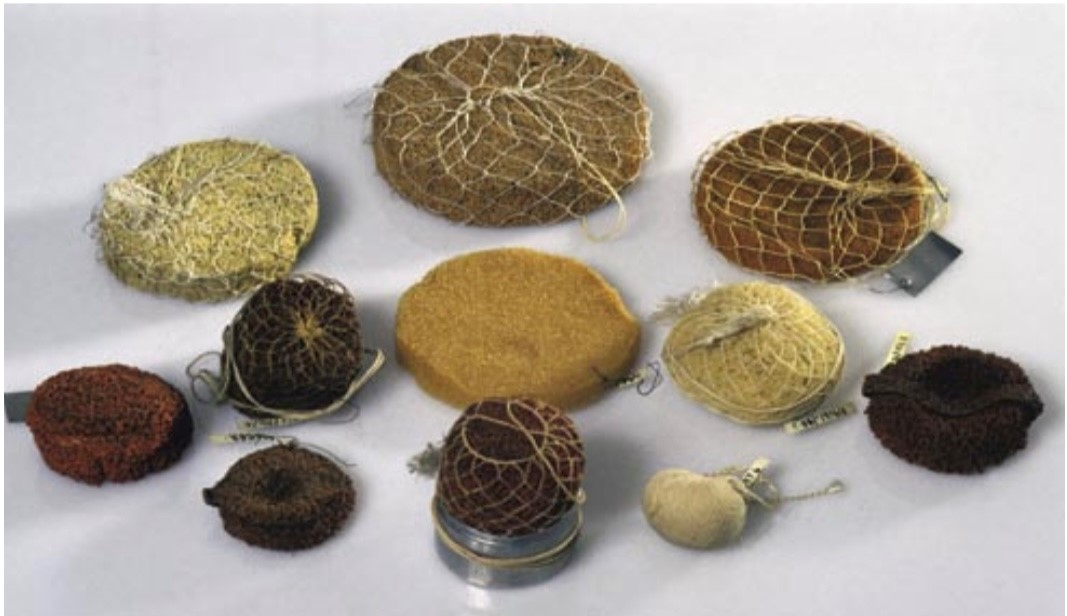
\includegraphics[scale=0.27]{Images/fig_9.jpg}
    \caption[short]{Éponges contraceptives du début du $20^e$ siècle fabriquées à partir de matériaux naturels et synthétiques.}
  \end{figure}
  
  \item \textbf{Les préservatifs: }Existants depuis des années, les préservatifs ont évolué de matériaux tels que les intestins d'animaux vers le latex et le polyuréthane modernes. Ils sont disponibles pour les deux sexes et demeurent une option populaire.


\begin{figure}[H]
    \centering
    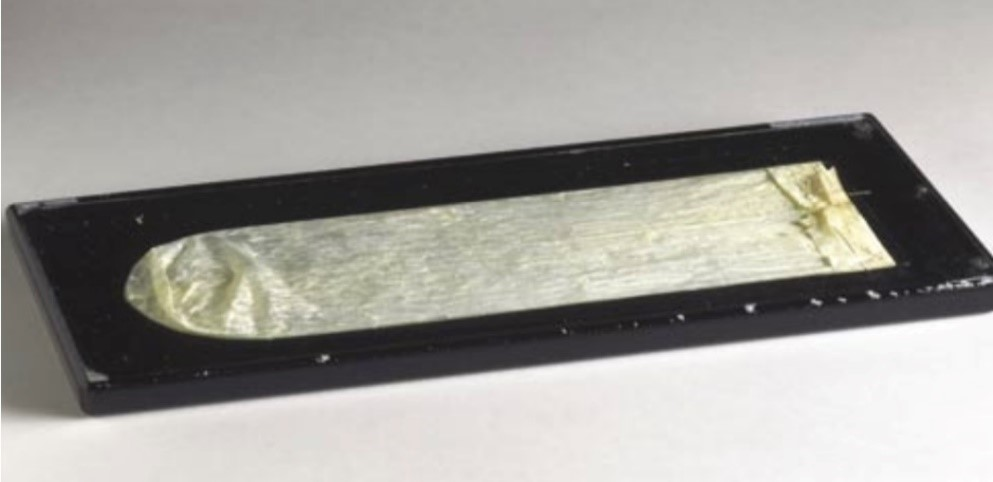
\includegraphics[scale=0.8]{Images/fig_10.jpg}
    \caption{Un préservatif masculin fait de membrane cæcale et de soie}
\end{figure}

\item \textbf{Les douches vaginales: }Utilisées autrefois pour éliminer les spermatozoïdes après les rapports, cette pratique a persisté, bien que son utilisation soit moins répandue aujourd'hui.

  \item \textbf{La contraception hormonale: }Initialement dérivées de tissus animaux, les hormones contraceptives sont désormais synthétiques. Cette méthode, largement répandue et efficace, a considérablement évolué au fil des années.

  \item \textbf{Les dispositifs intra-utérins: }Remontant à des matériaux tels que les intestins de vers à soie, les DIU modernes, notamment les stérilets, sont devenus des choix répandus et très efficaces pour la contraception.

  \item \textbf{La stérilisation: }Une méthode ancienne toujours en usage aujourd'hui, la stérilisation reste une option permanente pour ceux qui cherchent à éviter la conception.(14) 

\end{itemize}

\subsection{L’épidémiologie (statistiques démographiques): }
\noindent Entre 2015 et 2019, environ 121 millions de grossesses non désirées ont été recensées chaque année dans le monde, ce qui représente environ 48\% de l’ensemble des grossesses. Environ 61\% de ces grossesses ont été avortées. (15)\vspace*{1em}

\noindent L’Organisation des Nations Unies (ONU) estime qu’en 2050 la population mondiale se situera entre 9,4 et 10 milliards d’habitants, et la moitié des grossesses dans le monde ne sont pas désirées.(16) \vspace*{1em}

\noindent Selon Organisation Mondiale de la Santé, le nombre de femmes intéressées par la planification familiale a largement augmenté, passant de 900 millions en 2000 à environ 1,1 milliard en 2021. (17)\vspace*{1em}
  
\noindent En 2021, parmi les 1,9 milliard de femmes en âge de procréer dans le monde (15 à 49 ans), environ 1,1 milliard avaient besoin de services de planification familiales. Parmi elles, 874 millions utilisaient des méthodes de contraception modernes, tandis que 164 millions n’avaient pas accès à la contraception dont elles avaient besoin. (17)\vspace*{1em}

\noindent La proportion de femme en âge de procréer utilisant des méthodes modernes de planification familiale, est resté relativement stable à environ 77\% dans le monde entre 2015 et 2022. (17)\vspace*{1em}

\noindent En 2022, le taux global de prévalence de la contraception, toutes méthodes confondues, était estimé à 65\%, et le taux d’utilisation de méthodes contraceptives modernes par les femmes mariées ou en couple atteignait 58,7\%.(17)  \vspace*{1em}

\noindent En Afrique, en Asie et en Amérique latine, le nombre de naissances par femme était de 5 dans les années 1950, contre 2,5 aujourd’hui. L’utilisation de contraceptifs a également augmenté dans les pays en voie de développement passant de 9\% dans les années 1960 à 61\% actuellement. (18) \vspace*{1em}

\noindent Au Maroc, en 1979-1980, à peine une femme mariée sur cinq utilisait un moyen de contraception, mais en 2003-2004, plus de trois femmes mariées sur cinq y avaient recours. Entre 1962 et 2004, la fécondité a diminué progressivement, passant de 7 à 2,5 enfants par femme. (4) \vspace*{1em}

\noindent Dans les années 1960, le premier contraceptif injectable a été mis au point et c’est en 1969 que son utilisation a été approuvée. Environ 74 millions de femmes dans le monde utilisent des contraceptifs injectables en 2019, le DMPA étant le plus utilisé. (19) En Afrique subsaharienne, environ un tiers des utilisateurs de contraceptifs modernes ont recours à la contraception injectable intramusculaire. (20)\vspace*{1em}

\subsection{La stratégie nationale Marocaine dans le contrôle des naissances} 
Depuis le lancement du Programme National de Planification Familiale en 1966, des efforts considérables ont été déployés pour sensibiliser la population et répondre à ses besoins en planification familiale (PF). Plusieurs programmes ont été instaurés dans ce dessein, contribuant à élargir l'accès aux services de PF.\vspace*{1em}

\noindent Les prestation de PF sont désormais disponibles dans divers établissements de santé tels que les centres de santé, les dispensaires, les maternités, les centre de référence de PF, les cabinets médicaux et les cliniques. Une variété de professionnels de la santé, notamment des gynécologues, des chirurgiens, des médecins généralistes, et des sages - femmes, sont impliqués dans la prestation de ces services. \vspace*{1em}


\noindent Le dispositif intra-utérin, les contraceptifs oraux, les contraceptifs injectables, la contraception chirurgicale volontaire et les préservatifs figurent parmi les méthodes de PF disponibles, offrant ainsi un choix diversifié. (4) Ces méthodes sont accessibles à tous, qu'ils résident dans des zones urbaines ou rurales. (21) \vspace*{1em}  

\section{Les méthodes contraceptives }
Ce sont des méthodes naturelles ou artificielles utilisées pour prévenir une grossesse temporairement ou définitivement. Elles comprennent les méthodes naturelles, les méthodes locales, les méthodes hormonales et les méthodes chirurgicales. Cette diversité permet aux individus de choisir la méthode qui correspond le mieux à leurs besoins et à leur mode de vie.\vspace*{1em}

\subsection{Les méthodes naturelles}
Les méthodes contraceptives naturelles se distinguent par leur approche sans l'utilisation de matériel ou de produits médicaux qui interfèrent avec le système reproductif. Leur principe fondamental repose sur la compréhension et la détermination de la période de fertilité de la femme. (22) Toutefois, il est essentiel de reconnaître que ces méthodes peuvent présenter des défis, notamment lors de cycles menstruels irréguliers et chez les femmes en période péri-ménopausique, car les marqueurs d'ovulation deviennent plus difficiles à interpréter. (23)


Le retrait, également connu sous le nom de coït interrompu, se produit lorsque l'homme retire son pénis du vagin avant l'éjaculation dans le but d'éviter la fécondation.


\subsubsection{Le retrait (le coït interrompu)}
Cette méthode contraceptive est choisie par les couples désirant adopter une approche naturelle, améliorer l'efficacité d'autres méthodes contraceptives, ou encore lors de rapports sexuels occasionnels, acceptant un certain risque d'échec. Cependant, son utilisation est déconseillée dans les situations où l'homme n'est pas certain de pouvoir se retirer, en cas de risque élevé de maladies sexuellement transmissibles, et chez les femmes présentant des problèmes médicaux pour lesquelles une grossesse représente un risque important pour leur santé.\vspace*{1em}

\noindent L'efficacité du retrait repose en grande partie sur la détermination du couple à l'appliquer à chaque rapport sexuel. Les études montrent un taux d'échec estimé à 22\% dans une population donnée. Cependant, lorsque cette méthode est correctement maîtrisée par le couple, seulement 4\% des couples connaîtront une grossesse au cours des 12 mois suivants. (24)

\subsubsection{La méthode de l’allaitement maternel et de l’aménorrhée (MAMA)}
La MAMA est une option contraceptive à court terme, spécialement conçue pour les femmes récemment accouchées qui pratiquent l'allaitement exclusif. Elle peut être utilisée comme méthode contraceptive initiale avant de passer à d'autres méthodes plus durables.\\

\noindent L'efficacité de cette méthode repose sur le principe selon lequel l'allaitement fréquent inhibe la libération des hormones responsables de l'ovulation. Pour garantir une utilisation optimale, trois critères doivent être respectés:\vspace*{1em}

\begin{itemize}[label={$\bullet$}, align=right]
  \item Allaitement exclusif : La méthode MAMA fonctionne mieux lorsque la mère pratique un allaitement exclusif, sans recourir à d'autres sources de nutrition pour le nourrisson.

  \item Enfant âgé de moins de 6 mois : La méthode est recommandée jusqu'à ce que l'enfant atteigne l'âge de 6 mois. Après cette période, il est essentiel de mettre en place une autre méthode contraceptive pour maintenir une protection efficace.
  
  \item Aménorrhée chez la mère : La mère doit être aménorrhéique, c'est-à-dire ne pas avoir repris ses règles depuis l'accouchement.
  
\end{itemize}

\noindent Les études sur l'efficacité de la méthode MAMA ont révélé un taux de grossesse variant entre 0,45\% et 2,45\% à 6 mois. Des données provenant de six études non randomisées sur les utilisatrices de cette méthode ont montré un taux de grossesse allant de 0\% à 7,5\%. De plus, une étude prospective de l'Organisation Mondiale de la Santé sur l'aménorrhée de lactation et le retour de la fertilité a estimé un taux de grossesse d'environ 2\% à 6 mois. (25)

\begin{figure}[H]
  \centering
  
\includegraphics[scale=.5]{Images/fig_11.jpg}
  \caption{La méthode de l’allaitement maternel et de l’aménorrhée (26)}
\end{figure}

\subsubsection{La méthode du calendrier }
La méthode du calendrier, également connue sous le nom de méthode Ogino-Knauss, a été élaborée dans les années 1920 par Kyusaku Ogino et Herman Knaus. Elle propose une approche simple, demandant aux femmes de surveiller la durée de leur cycle menstruel afin de déterminer leurs jours de fertilité, pendant lesquels elles doivent pratiquer l'abstinence.\\

\noindent Les jours considérés comme fertiles se situent généralement entre le 12e et le 19e jour du cycle menstruel, bien que cette plage puisse varier en fonction de la durée du cycle individuel. Il est important pour les utilisatrices de comprendre la variation potentielle en fonction de leur propre cycle. \\

\noindent Cependant, des études récentes ont mis en évidence des limitations dans l'efficacité de cette méthode. Une méta-analyse portant sur huit études a révélé un taux de 15 à 18 grossesses pour 100 utilisatrices standardisées sur une période d'observation de 12 mois. Ces résultats soulignent la nécessité pour les femmes de considérer d'autres méthodes contraceptives plus fiables. (27) \\

\begin{figure}[H]
  \begin{center}
    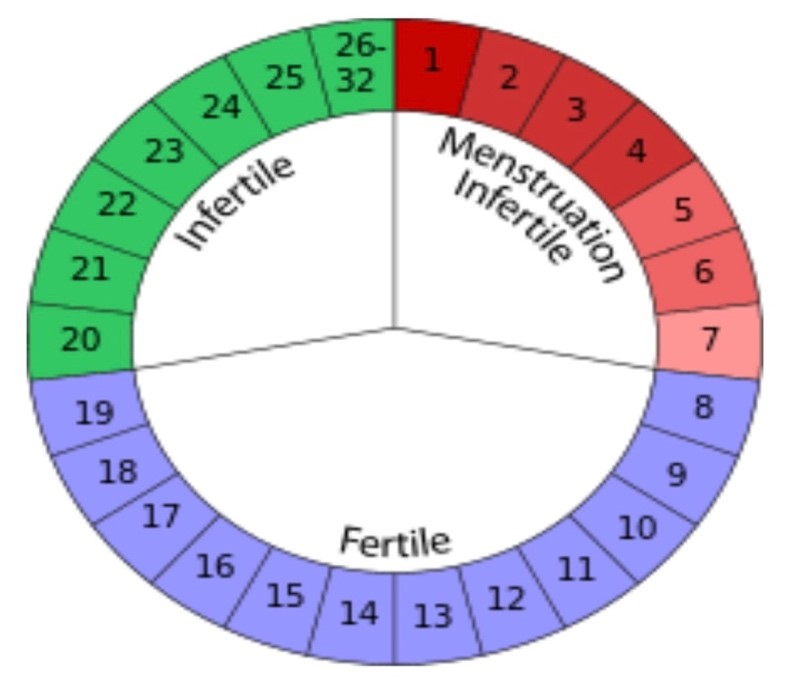
\includegraphics[scale=.8]{Images/fig_12.jpg}
    \caption{La méthode Ogino Knauss (28)}
  \end{center}
\end{figure}

\subsubsection{La méthode des deux jours}
Cette approche repose sur l'observation de la glaire cervicale pour déterminer les jours fertiles. Lorsque la glaire est présente pendant deux jours consécutifs, la fertilité est élevée. Si la glaire est présente uniquement un jour, ce jour est également considéré comme fertile. Cependant, en l'absence de glaire cervicale pendant deux jours consécutifs, la probabilité de fertilité est jugée faible. (22)\\

\subsubsection{La méthode des jours fixes}
Cette approche vise à prévenir une grossesse en évitant les rapports sexuels non protégés pendant les jours fertiles. Elle repose principalement sur l'abstinence sexuelle ou l'utilisation d'une méthode de contraception barrière, spécifiquement du 8e au 19e jour du cycle menstruel, pour les femmes dont leur cycle dure entre 26 et 32 jours. (22) 

\begin{figure}[H]
  \centering
  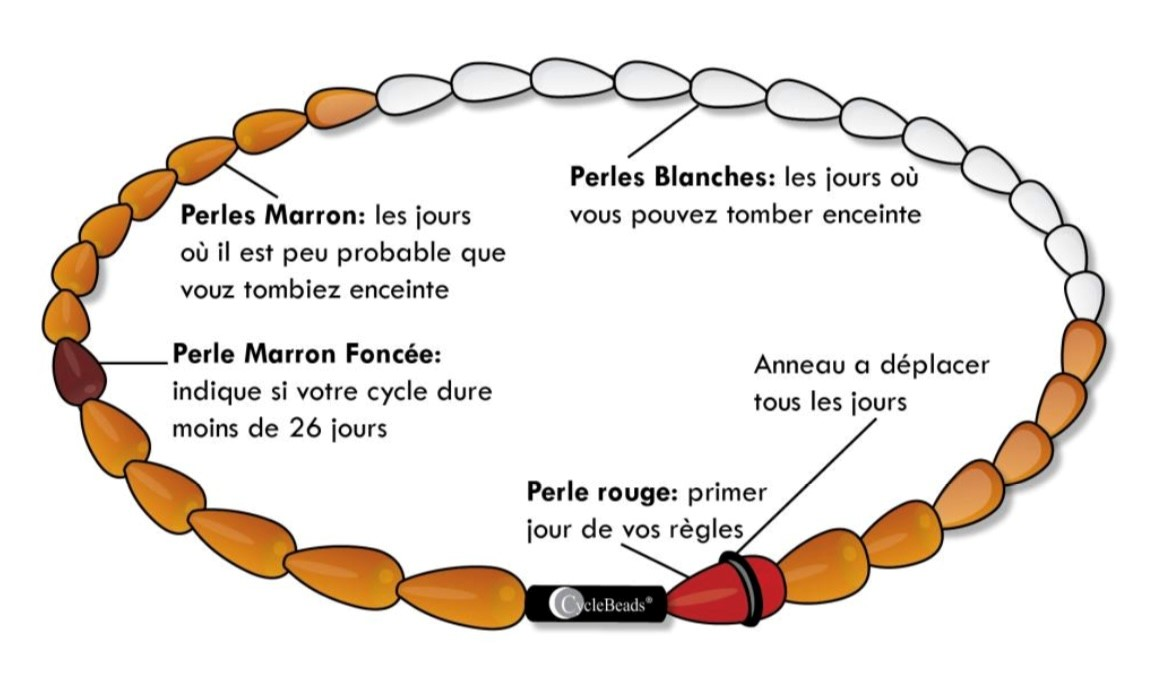
\includegraphics[scale=.3]{Images/fig_13}
  \caption{La méthode des jours fixes (29)}
\end{figure}

\subsubsection{La méthode de l’observance de la glaire cervicale}
Cette méthode, également nommée la méthode Billings, repose sur l’observation de la glaire cervicale pour permettre à la femme de déterminer sa période de fertilité. (30) \\

\noindent Il est important de noter que les rapports sexuels au cours des 5 jours précédant l'ovulation et le jour de l'ovulation présentent un risque significatif de grossesse. Pendant cette période, les sécrétions de la glaire cervicale augmentent en raison de la stimulation par l'augmentation des œstrogènes.\\

\noindent Une étude a révélé que la probabilité de conception les jours sans sécrétions est d'environ 0,3\%, tandis qu'elle est d'environ 30\% les jours où des sécrétions fertiles sont présentes. (31) 

\begin{figure}[H]
  \centering
  
\includegraphics[scale=.3]{Images/fig_14.jpg}
  \caption{La méthode Billings (28)}
\end{figure}

\subsubsection{La méthode de la température :}
Également appelée "méthode de la température basale", cette approche implique la prise de la température corporelle au repos chaque matin, idéalement à la même heure. La méthode repose sur le principe que la température corporelle augmente après l'ovulation en raison de l'augmentation de la progestérone, signifiant la fin de la période de fertilité. Pour éviter la conception, la femme s'abstiendra de rapports sexuels pendant les trois premiers jours suivant cette augmentation de la température. (22) (32) \\

\noindent Cependant, il convient de noter que cette méthode présente des limitations en raison des influences exogènes sur la température des femmes, telles que le stress, la fièvre, et d'autres facteurs. (33)\\

\begin{figure}[H]
  \centering
  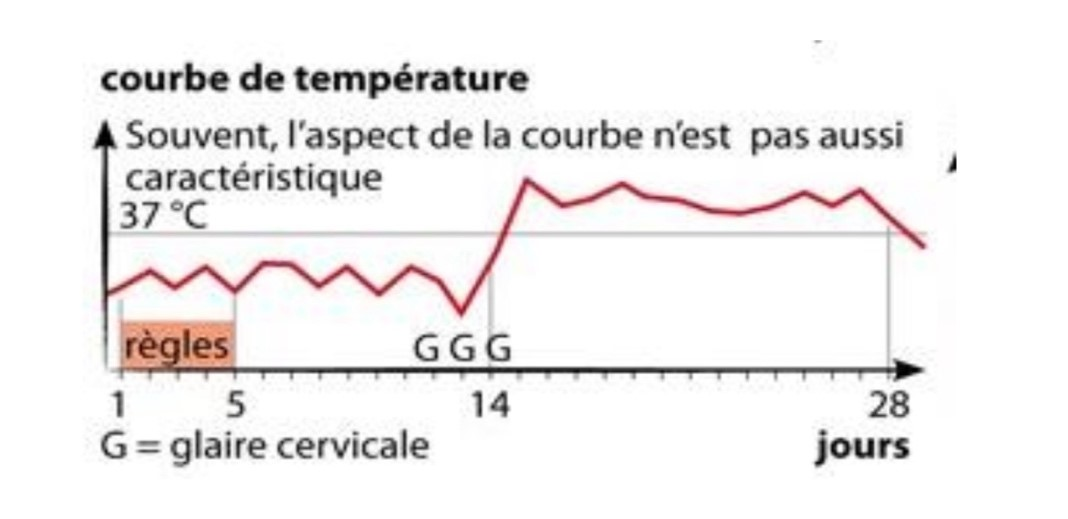
\includegraphics{Images/fig_15.jpg}
  \caption{La méthode des températures (28)}
\end{figure}

\subsubsection{La méthode symptothermique}
Il s’agit d’une méthode contraceptive qui est basée à la fois sur la méthode des températures et sur la méthode d’observation de la glaire cervicale. Les couples l'adoptent pour déterminer avec précision leur période de fertilité, en observant la température basale du corps ainsi que la texture et la quantité de la glaire cervicale. Ces informations permettent des choix éclairés pour éviter une grossesse non désirée.\\

\noindent Durant la période fertile, la température basale est notablement élevée, accompagnée d'une glaire cervicale abondante, claire, liquide et filante. En revanche, pendant la période infertile, la température basale diminue et la glaire cervicale devient plus épaisse et collante.\\

\noindent Il est intéressant de noter qu'une tendance à la hausse est observée depuis 1970 parmi les utilisatrices de cette méthode, avec une augmentation moyenne de 3 à 4\%. (34)\\ 

\begin{figure}[H]
  \centering
  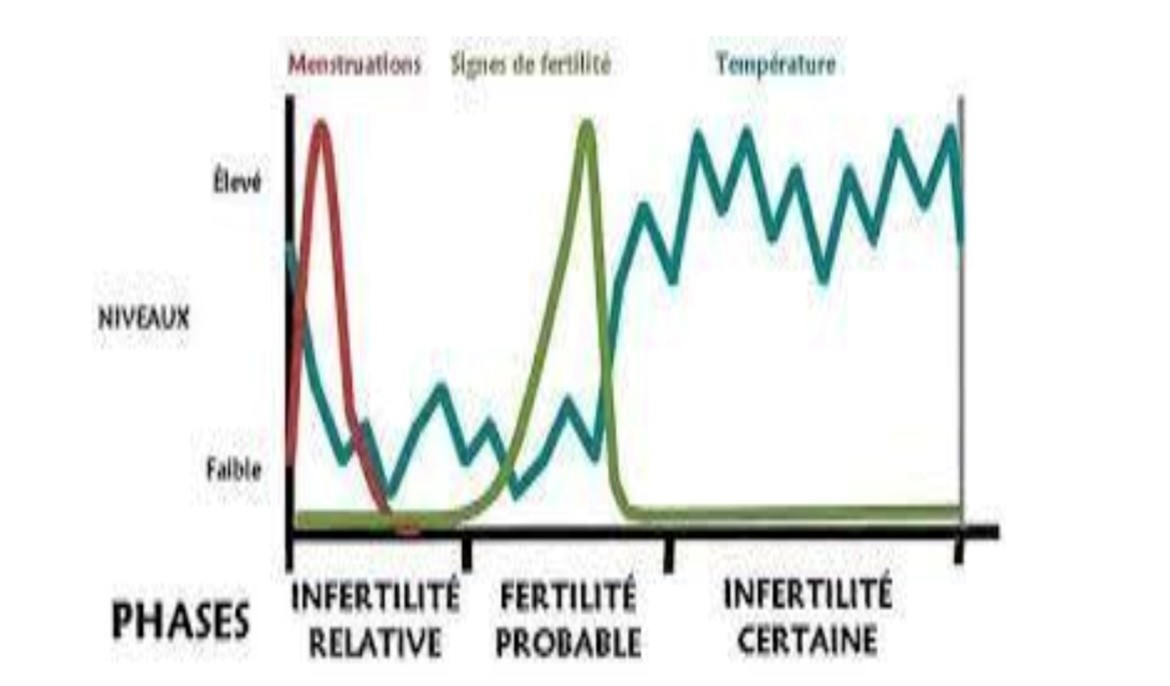
\includegraphics[scale=.3]{Images/fig_16.jpg}
  \caption{La méthode symptothermique(28)}
\end{figure}

\subsubsection{Le suivi de la fertilité utilisant des moniteurs de fertilité}
L'utilisation croissante des moniteurs de fertilité témoigne de l'intérêt grandissant des femmes pour une alternative à la contraception hormonale. Des études ont démontré que l’efficacité de cette méthode peut être aussi élevée que celle de la contraception hormonale lorsqu’elle est correctement utilisée. \\

\noindent Ces dispositifs permettent aux femmes de surveiller leur cycle menstruel en mesurant divers paramètres tels que l'augmentation de l'œstrogène dans l'urine avant l'ovulation, la présence de l'hormone lutéinisante, la température basale, etc. Cependant, il est important de noter que ces appareils peuvent être complexes à utiliser et sont parfois coûteux. (35) (36)   \\

\noindent Pendant la période de fertilité ainsi identifiée, les femmes ont le choix de s'abstenir de rapports sexuels ou d'opter pour d'autres méthodes contraceptives, telles que l'utilisation de préservatifs. \\

\begin{figure}[H]
  \centering
  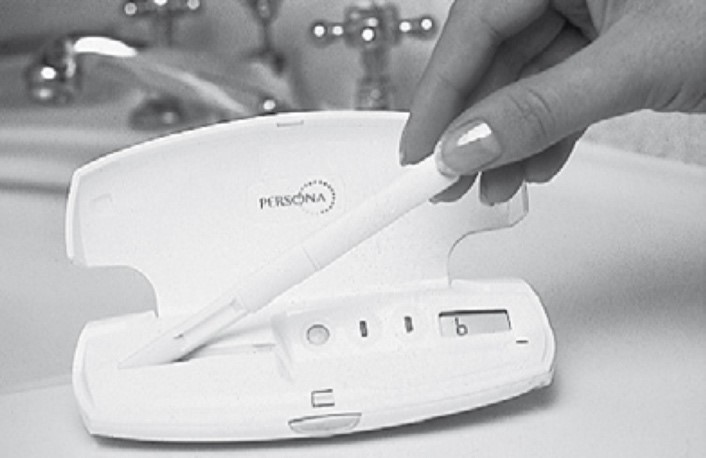
\includegraphics{Images/fig_17.jpg}
  \caption{Moniteur de fertilité (37)}
\end{figure}

\subsection{Les méthodes locales}

\subsubsection{Les préservatifs:}

\noindent Les préservatifs sont des dispositifs contraceptifs utilisés pour prévenir les grossesses en agissant comme une barrière efficace contre la pénétration du sperme. De manière notable, ils représentent également le seul moyen de contraception qui offre une protection contre les infections sexuellement transmissibles. \\

\noindent Il existe des préservatifs masculins et féminins. Ils sont généralement en latex. Toutefois, pour les individus allergiques au latex, des alternatives telles que le polyuréthane ou le nitrile, reconnus pour leur caractère hypoallergénique, sont disponibles. Ces dispositifs se déclinent dans une variété de textures, couleurs, tailles, formes, sensations et parfums. Certains sont également dotés de spermicides ou de lubrifiants.\\

\noindent Les préservatifs sont très efficaces lorsqu’ils sont utilisés correctement. Le taux d’efficacité des préservatifs masculins est de 98\% et celui des préservatifs féminins de 95\%.(38) Les couples qui utilisent le préservatif comme principal moyen de contraception ont un taux de grossesse situé entre 15 à 20\% par an. (39) 

\begin{figure}[H]
  \centering
  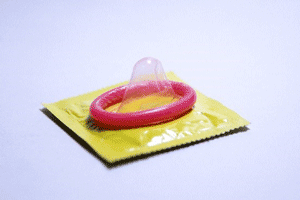
\includegraphics[scale=.7]{Images/fig_18b.jpg}
  \caption{Préservatif masculin (40)}
\end{figure}

\begin{figure}[H]
  \centering
  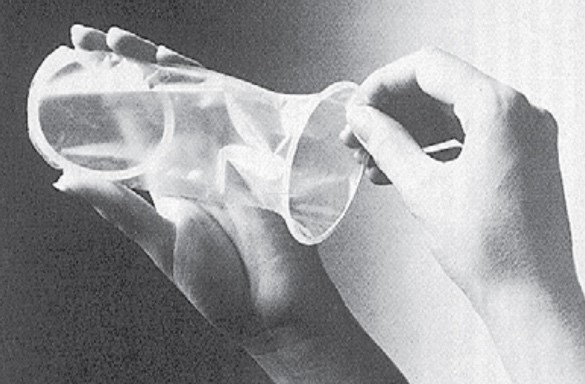
\includegraphics[scale=1]{Images/fig_19.jpg}
  \caption{Préservatif féminin (41)}
\end{figure}

\subsubsection{Les spermicides:}
\noindent Un spermicide est une méthode locale de contraception qui inactive ou tue les spermatozoïdes, empêchant ainsi la grossesse. Il est utilisé en complément d’autres méthodes contraceptives telles que les diaphragmes, les préservatifs, etc. Pour qu’il soit complètement absorbé, il doit être utilisé 10 minutes avant le rapport sexuel. Il se présente sous différentes formes galéniques (gels, crèmes, éponges, ovules, etc.). Ils peuvent être naturels ou chimiques, les deux principales molécules étant le nonoxynol-9 et le chlorure de benzalkonium. (42)\\

\noindent \textbf{Les indications des spermicides sont les suivantes :}
\begin{itemize}[label={$\bullet$}, align=right]
  \item Comme méthodes supplémentaires de contraception lors de l’utilisation :
  \begin{itemize}[label={$\circ$}]
    \item Des méthodes barrières de contraception,
    \item Des méthodes de contraception naturelles, 
    \item De contraceptifs oraux en cas d’oubli.
  \end{itemize}  

  \item Comme méthode principale de contraception chez :
  \begin{itemize}[label={$\circ$}]
    \item Les couples souhaitant seulement espacer leurs enfants,
    \item	Les femmes de plus de 45 ans,
    \item Les couples hypofertiles,
    \item Les femmes en post-partum, mais les spermicides à base de nonoxynol-9 doivent être évités pendant l’allaitement,
    \item Les couples ayant des activités sexuelles peu fréquentes,
    \item	En cas de contre-indications aux stérilets et aux pilules.  
  \end{itemize}
\end{itemize}\vspace*{1em}

\noindent \textbf{Les contre-indications des spermicides sont les suivantes :}
\begin{itemize}[label={$\bullet$}, align=right]
  \item Allergie locale aux spermicides,
  \item	Les couples qui ne veulent pas d’enfants,
  \item	Risque de contracter le VIH ou d’autres infections sexuellement transmissibles,
  \item	Les adolescentes et les jeunes femmes,
  \item	Couples sexuellement très actifs. 
\end{itemize} \vspace*{1em}

\noindent \textbf{Les avantages des spermicides sont : }
\begin{itemize}[label={$\bullet$}, align=right]
  \item Ils ne présentent pas de risque majeur pour la santé,
  \item C’est une méthode de contraception occasionnelle,
  \item Ils ne nécessitent pas de prescription médicale, 
  \item Ils donnent à la femme la possibilité de prendre en charge la contraception, 
  \item Certains spermicides ont des effets lubrifiants.
\end{itemize} \vspace*{1em}

\noindent \textbf{Les inconvénients des spermicides sont les suivantes :}

\begin{itemize}[label={$\bullet$}, align=right]
  \item Ils peuvent provoquer des allergies locales,  
  \item Ils ne sont pas très efficaces, 
  \item Ils doivent être utilisés à chaque rapport sexuel, 
  \item Ils sont chers,
  \item Ils nécessitent que la femme connaisse son appareil génital, 
  \item Certains spermicides ont un délai avant le début de leur efficacité,
  \item Ils sont peu acceptés, 
  \item Certains spermicides coulent excessivement. (41)
\end{itemize} \vspace*{1em}

\begin{figure}[H]
  \centering
  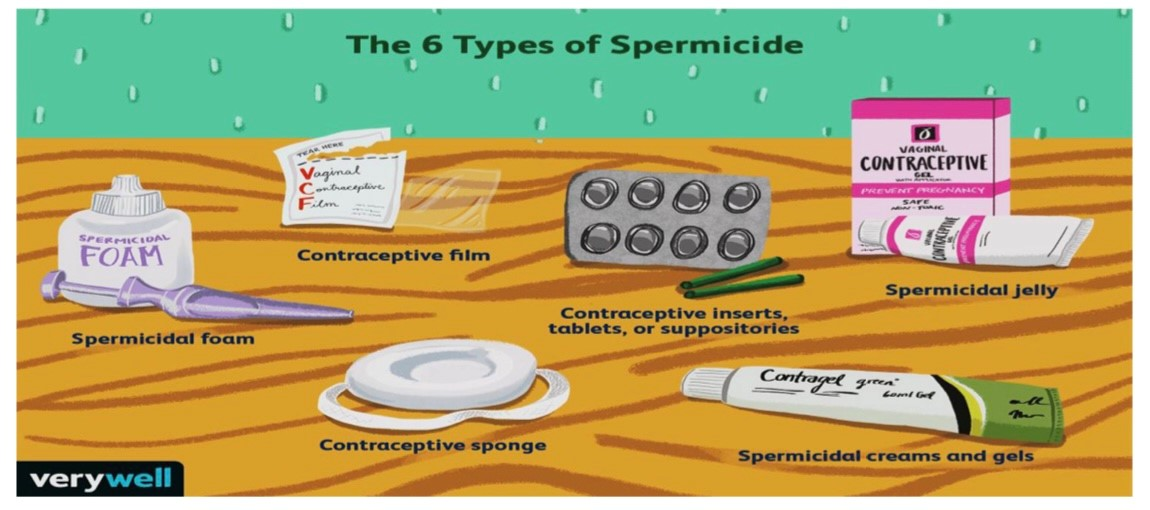
\includegraphics[scale=.4]{Images/fig_20.jpg}
  \caption{Les spermicides (40)}
\end{figure}

\noindent En France et dans d’autres pays européens, 2 à 6\% des couples utilisent des spermicides comme moyen de contraception. Pour les spermicides utilisés correctement, le taux d’échec théorique est compris entre 0 et 7,6\%. (43)  

\subsubsection{Le diaphragme :}
\noindent  C’est le premier moyen de contraception moderne fiable pour les femmes qui empêche les spermatozoïdes de traverser le col de l’utérus. (41)  Il s’agit d’un dispositif contraceptif qui peut s’avérer très efficace lorsqu’il est utilisé avec un spermicide. Il protège modérément contre les infections sexuellement transmissibles mais présente un risque d’infection des voies urinaires et de syndrome de choc toxique. (44) \\

\noindent \textbf{L’indication des diaphragmes est la suivante :}

\begin{itemize}[label={$\bullet$}, align=right]
\item  Les femmes désirant une méthode de contraception vaginale efficace et peu couteuse.
\end{itemize}\vspace*{1em}

\noindent \textbf{Les contre-indications des diaphragmes sont :}
\begin{itemize}[label={$\bullet$}, align=right]
  \item  Les femmes allergiques aux latex ou aux spermicides. 
  \item  Les femmes présentant des infections urinaires répétées. 
  \item	Anatomiques: 
  \begin{itemize}[label={$\circ$}]
    \item Périnée déficiente, 
    \item Fibrome postérieur, 
    \item Prolapsus génital important, 
    \item	Vagin plat de type juvénile, 
    \item	Rétroversion utérine fixée. 
  \end{itemize}
\end{itemize}\vspace*{1em}

\noindent \textbf{Les avantages des diaphragmes sont :}

\begin{itemize}[label={$\bullet$}, align=right]
  \item Ils peuvent être utilisés à tout âge, 
  \item	Ils préviennent modérément les infections sexuellement transmissibles,
  \item	Ils ne sont pas chers, 
  \item	Ils peuvent être placés discrètement, 
  \item Ils nécessitent un examen gynécologique, ce qui permet dépistage et suivi, 
  \item	Ils ne présentent pas de contre-indications (sauf anatomiques).
\end{itemize}\vspace*{1em}

\noindent \textbf{Les inconvénients des diaphragmes sont:}

\begin{itemize}[label={$\bullet$}, align=right]
  \item Une consultation médicale préalable est obligatoire,
  \item Les infections urinaires sont plus fréquentes chez les utilisatrices que chez les non utilisatrices,
  \item Le taux d’échec est élevé,
  \item Ils sont encombrants,
  \item Les utilisatrices nécessitent un apprentissage auprès de professionnels de la santé formés,
  \item Ils sont mal acceptés par les jeunes,
  \item Ils n’empêchent pas la transmission sexuelle du VIH. (41)  

\end{itemize}

\begin{figure}[H]
  \centering
  \begin{subfigure}[b]{0.45\textwidth}
      \centering
      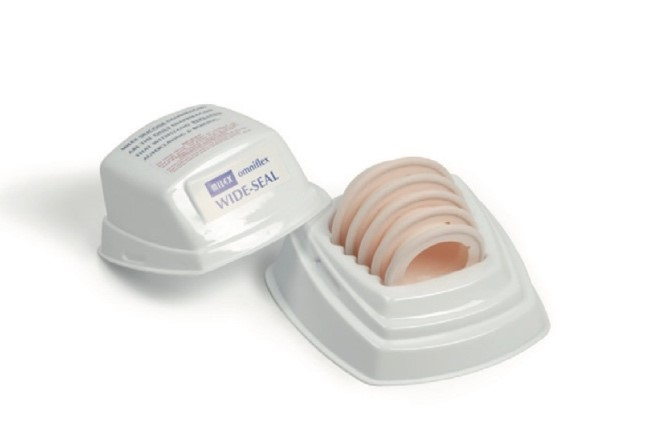
\includegraphics[width=\textwidth]{Images/fig_21a.jpg}
      % \caption{Caption for Image 1}
      % \label{fig:image1}
  \end{subfigure}
  \hfill
  \begin{subfigure}[b]{0.45\textwidth}
      \centering
      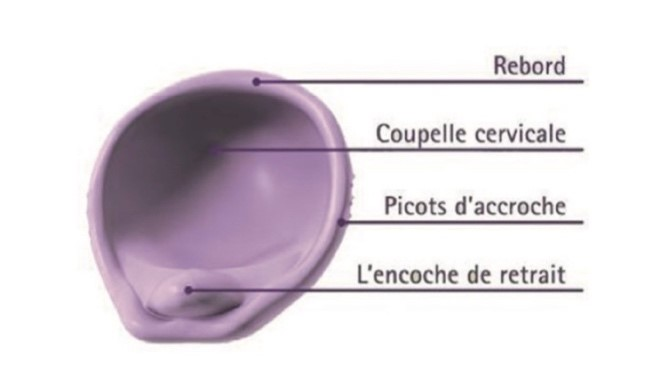
\includegraphics[width=\textwidth]{Images/fig_21b.jpg}
      % \caption{Caption for Image 2}
      % \label{fig:image2}
  \end{subfigure}
  \caption{Diaphragmes (45)}
  % \label{fig:both_images}
\end{figure}

\subsubsection{La cape cervicale :}

\noindent Elle constitue une forme de contraception féminine de type barrière. Il s’agit d’un dispositif contraceptif, une cupule en silicone ou en latex placée dans le vagin pour empêcher les spermatozoïdes d’atteindre l’ovule. Pour une meilleure efficacité, elle est utilisée avec un spermicide. Elle doit être mise en place avant le rapport sexuel et doit être laissée en place pendant au moins six heures avant de la retirer. Elle est réutilisable, mais doit être lavée avec un savon doux, séchée et conservée correctement. (22)

\begin{figure}[H]
  \centering
  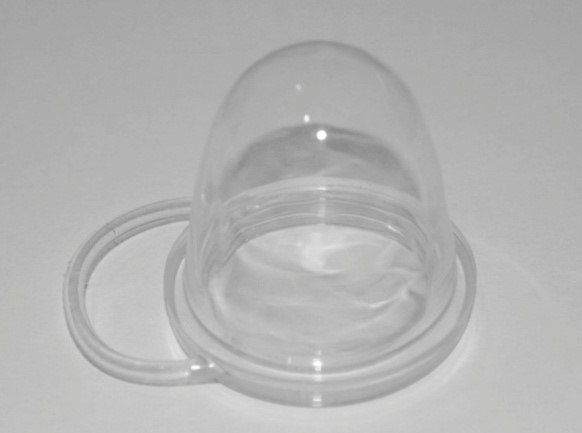
\includegraphics{Images/fig_22.jpg}
  \caption{Cape cervicale (46)}
\end{figure}

\subsubsection{L’éponge contraceptive: }
Il s’agit d’une méthode de contraception de type barrière. Elle est utilisée avec un spermicide pour être efficace. Elle recouvre le col de l’utérus et, grâce au spermicide, empêche les spermatozoïdes de pénétrer dans l’utérus.\\

\noindent \textbf{Les avantages de cette méthode sont les suivants:}

\begin{itemize}[label={$\bullet$}, align=right]
  \item	Elle est contrôlée par la femme,
  \item Elle ne contient pas d’hormones et ne présente donc pas d’effets indésirables hormonaux, 
  \item Elle ne nécessite pas de prescription médicale,
  \item	Elle ne coûte pas cher, 
  \item Il n’est pas nécessaire d’ajouter du spermicide lorsque l’éponge est réutilisée dans les 24 heures. (47)
\end{itemize}

\noindent \textbf{Les indications l’éponge contraceptive au chlorure de benzalkonium sont:}

\begin{itemize}[label={$\bullet$}, align=right]
  \item Les couples ayant des rapports sexuels peu fréquents,
  \item	Femmes de plus de 45 ans,  
  \item Contraception temporaire dans l’attente d’une contraception définitive, 
  \item Couples désirant une méthode contraceptive locale sans écoulement excessif de spermicide, 
  \item	Femmes en post-partum. 
\end{itemize}

\noindent \textbf{Les contre-indications de l’éponge contraceptive au chlorure de benzalkonium sont:}
\begin{itemize}[label={$\bullet$}, align=right]
  \item Femmes allergiques au spermicide chlorure de benzalkonium, 
  \item L’incapacité d’utiliser correctement cette méthode, 
  \item Déficience périnéale ou prolapsus génital, 
  \item Femmes sexuellement actives et fertiles. (41) 
\end{itemize}

\begin{figure}[H]
  \centering
  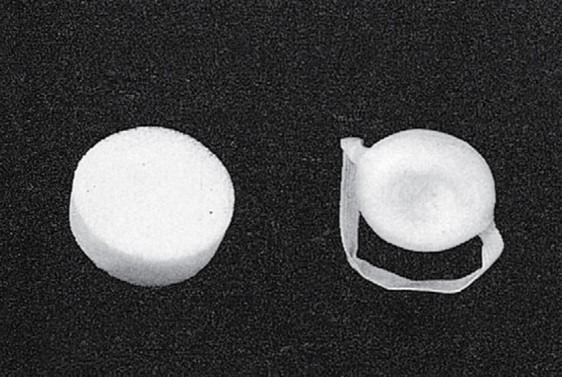
\includegraphics{Images/fig_23.jpg}
  \caption{Éponge contraceptive (41)}
\end{figure}

\subsubsection{Les dispositifs intra-utérins:}
\noindent Ils sont également connus sous le nom de stérilet et constituent le moyen de contraception le plus utilisé dans le monde. (48) Il s’agit d’une contraception à long terme, de 3 à 10 ans selon le type utilisé. Il en existe deux types, les DIU hormonaux et les DIU non hormonaux. Pour les dispositifs non hormonaux, on trouve le DIU au cuivre et pour les dispositifs hormonaux, on trouve le DIU à libération de lévonorgestrel. (49) \\

\noindent C’est un moyen de contraception très efficace avec un taux d’échec très faible de 0,3\% pour les DIU hormonaux et de 0,6 à 0,8\% pour les DIU au cuivre. (50)

\subsubsection{Les dispositifs intra-utérins hormonaux:}
\noindent Ils sont également connus sous le nom de système intra-utérin au lévonorgestrel. Leur mécanisme d’action consiste à inhiber l’ovulation et à bloquer le développement de l’endomètre. Ils inhibent également la fonction des spermatozoïdes et modifient la muqueuse endométriale pour empêcher la nidation. (10)\\

\noindent En plus de leur utilisation contraceptive, ils présentent des avantages non contraceptifs qui sont les suivants : 

\begin{itemize}[label={$\bullet$}, align=right]
  \item Ils permettent de prévenir et traiter l’hyperplasie et le cancer de l’endomètre, 
  \item	Ils aident à lutter contre l’anémie, 
  \item Ils permettent de lutter contre la ménorragie,
  \item Ils aident à traiter l’adénomyose et les fibromes, 
  \item Ils permettent de traiter l’endométriose,
  \item Ils peuvent réduire le risque de maladie inflammatoire pelvienne. (51)
\end{itemize}

\begin{figure}[H]
  \centering
  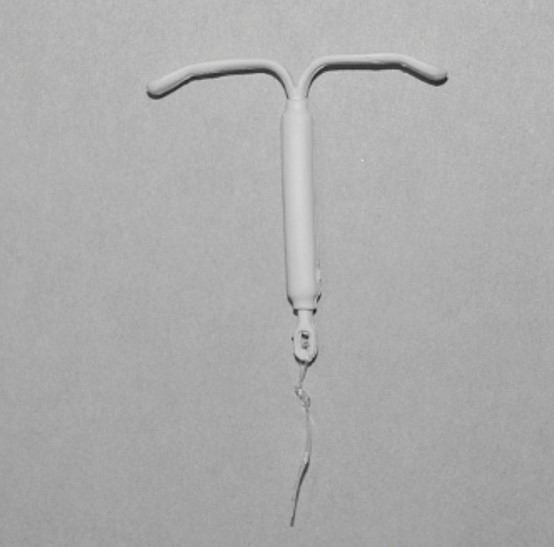
\includegraphics{Images/fig_24.jpg}
  \caption{Dispositif intra-utérin hormonal (46)}
\end{figure}

\subsubsection{Les dispositifs intra-utérins au cuivre:}

\noindent C’est une méthode de contraception non hormonale. Il s’agit d’un dispositif en plastique autour duquel est enroulé un fil de cuivre. Son mécanisme d’action est l’inhibition de l’implantation par l’effet cytotoxique du cuivre sur les spermatozoïdes. (11) Il a un effet sur la glaire cervicale empêchant la pénétration des spermatozoïdes et empêchent l’implantation par sa réponse inflammatoire sur l’endomètre. (52) 

\begin{figure}[H]
  \centering
  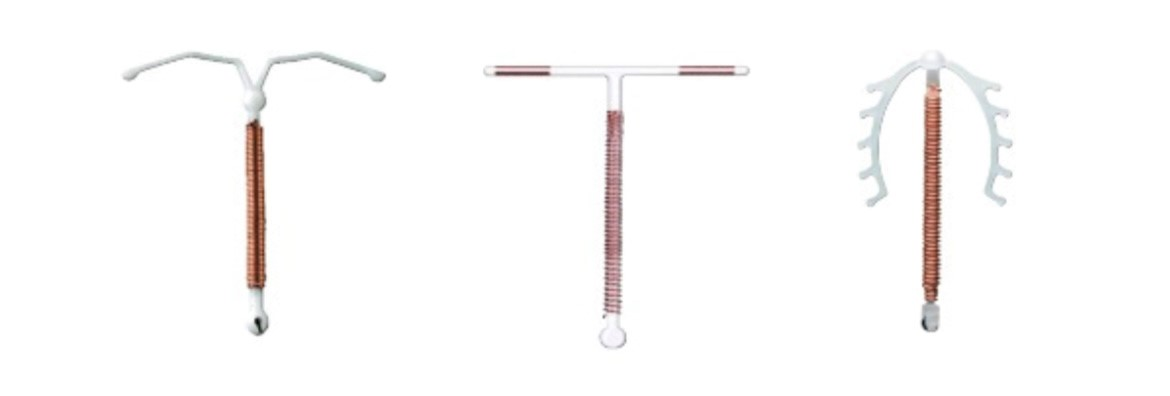
\includegraphics[scale=0.4]{Images/fig_25.jpg}
  \caption{Dispositifs intra-utérins au cuivre (53)}
\end{figure}

\noindent Cependant, bien qu’il s’agisse de l’une des méthodes de contraception les plus efficaces, elle n’est pas exempte d’inconvénients. Ces inconvénients sont notamment : 

\begin{itemize}[label={$\bullet$}, align=right]
  \item	L’expulsion du dispositif, 
  \item La douleur lors de la pose ou du retrait, 
  \item	Les ménorragies,
  \item	Les infections. (48)  
\end{itemize}

\noindent Les contre-indications absolues de cette méthode sont indiquées dans le tableau ci-dessous :

\begin{table}[H]
  \centering
  \begin{tabular}{c}
      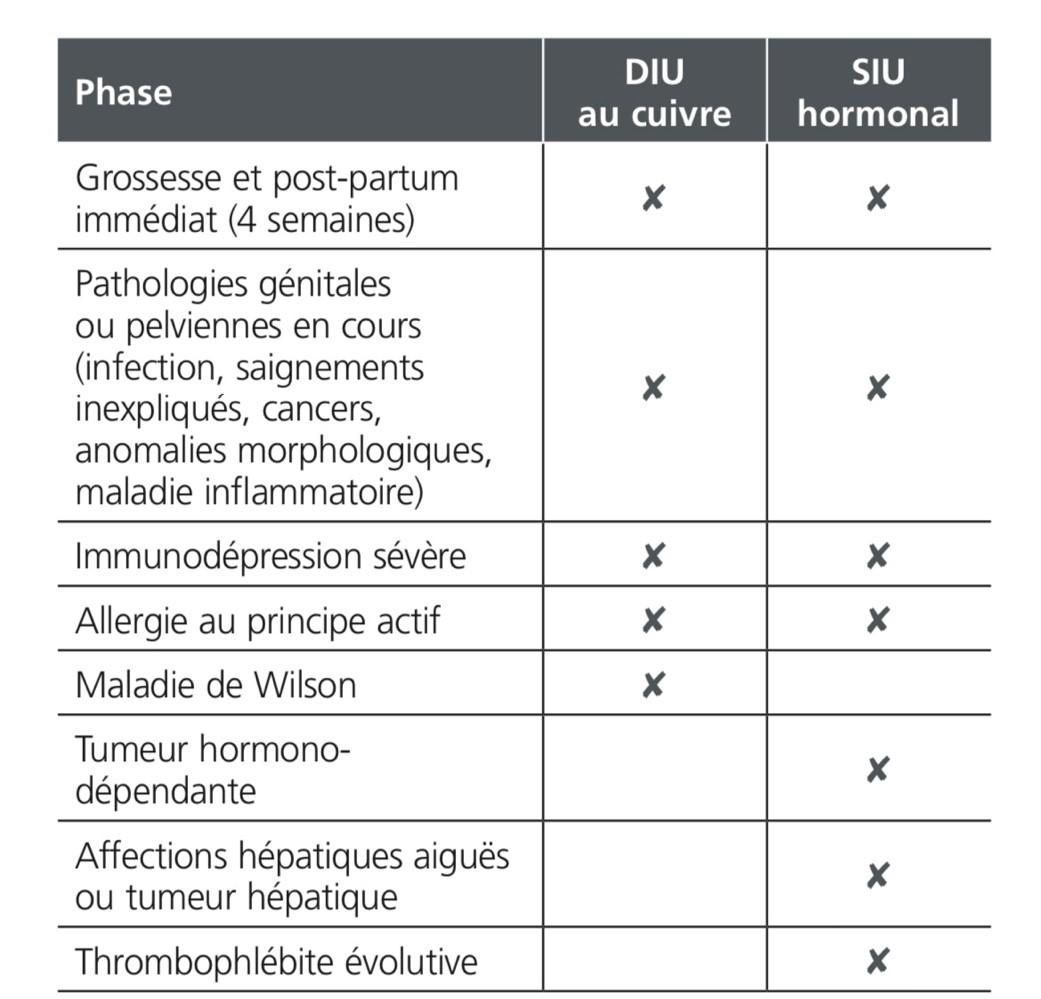
\includegraphics{Images/tab_1.jpg} \\
  \end{tabular}
  \caption{Les contre-indications absolues des dispositifs intra-utérins(53)}
  % \label{tab:contra_indications}
\end{table}

\subsection{Les méthodes hormonales:}

\noindent Les contraceptifs hormonaux sont utilisés depuis des décennies dans le monde entier pour la contraception. Ils contiennent tous un progestatif. (54) Ils agissent en inhibant l’ovulation et en modifiant la glaire cervicale, bloquant ainsi la pénétration des spermatozoïdes. (55)  Il en existe différents types comme les contraceptifs oraux, les contraceptifs injectables, les implants sous-cutanés, les stérilets, etc. Ces méthodes agissent en libérant des hormones contraceptives dans le corps.\\  

\noindent Les hormones utilisées dans la contraception hormonale sont les progestatifs et l’éthinyl estradiol.\\

\noindent \textbf{Le progestatif} est la forme synthétique de l’hormone progestérone. Ils sont utilisés pour la contraception seule ou avec l’œstrogène. Ils peuvent être classés en fonction de leur génération ou leur structure. (56)\\

\noindent Les quatre générations de progestatifs sont les suivantes : 

\begin{itemize}[label={$\bullet$}, align=right]
  \item \textbf{Première génération:} Noréthistérone
  \item \textbf{Deuxième génération:} Noréthistérone
  \item \textbf{Troisième génération:} Noréthistérone
  \item \textbf{Quatrième génération:} Drospirénone, Acétate de chlormadinone, Diénogest (10)  
\end{itemize}

\noindent D’un point de vue structurel, les progestatifs utilisés pour la contraception sont: 

\begin{itemize}[label={$\bullet$}, align=right] 
  \item Les dérivés de la testostérone tels que : 
  \begin{itemize}[label={$\circ$}]
    \item Le lévonorgestrel
    \begin{figure}[H]
      \centering
      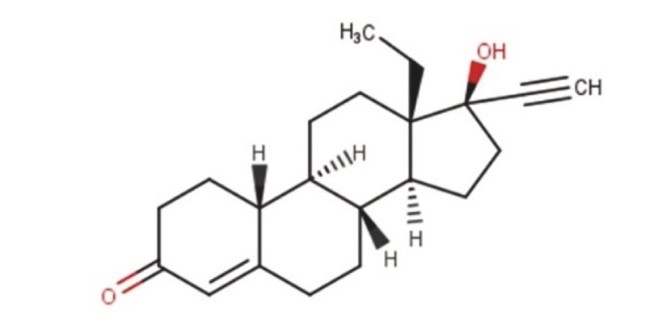
\includegraphics{Images/fig_26.jpg}
      \caption{Le lévonorgestrel (57)}
    \end{figure}
    \item La noréthistérone 
    \begin{figure}[H]
      \centering
      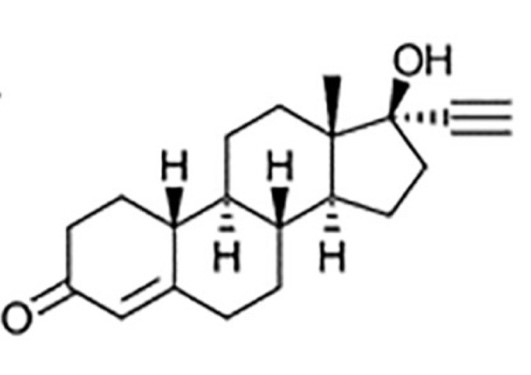
\includegraphics{Images/fig_27.jpg}
      \caption{La noréthistérone (58)}
    \end{figure}

    \item L’acétate de chlormadinone 
    \begin{figure}[H]
      \centering
      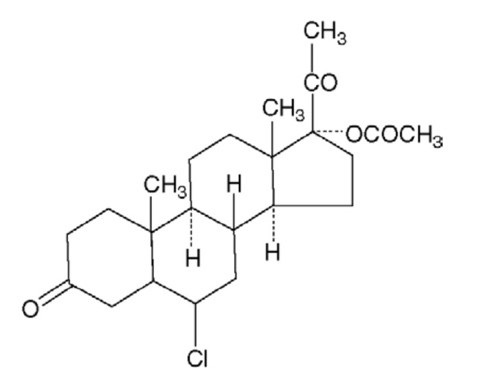
\includegraphics{Images/fig_28.jpg}
      \caption{Acétate de chlormadinone (59)}
    \end{figure}

  \end{itemize}

  \item Les dérivés du norgestrel : Ce sont des anti-gonadotropes tels que:
  \begin{itemize}[label={$\circ$}] 
    \item Norgestimate 
    \begin{figure}[H]
      \centering
      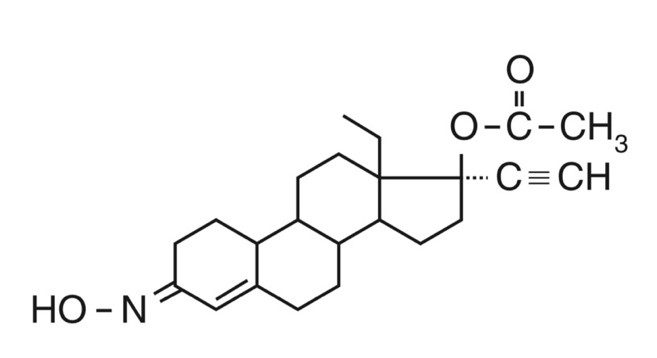
\includegraphics{Images/fig_29.jpg}
      \caption{Norgestimate (60)}
    \end{figure}
    \item Gestodène 
    \begin{figure}[H]
      \centering
      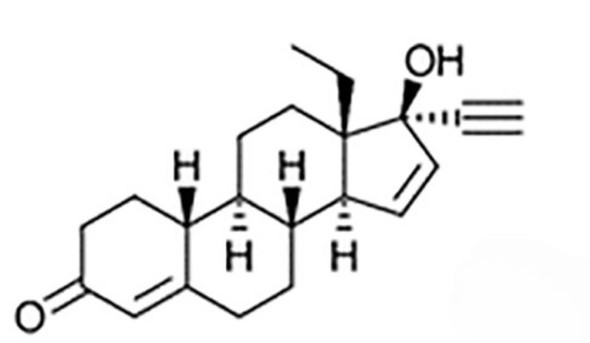
\includegraphics{Images/fig_30.jpg}
      \caption{Gestodène (58)}
    \end{figure}
    \item Désogestrel
  \end{itemize}
  \item Le dérivé de la spironolactactone : La drospirénone 
  \begin{figure}[H]
    \centering
    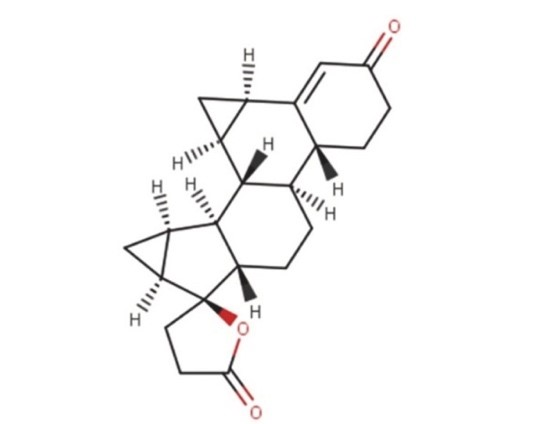
\includegraphics{Images/fig_31.jpg}
    \caption{Drospirenone (57)}
  \end{figure}

  \item Norelgestromine : C’est un précurseur du norgestrel. 
  \begin{figure}[H]
    \centering
    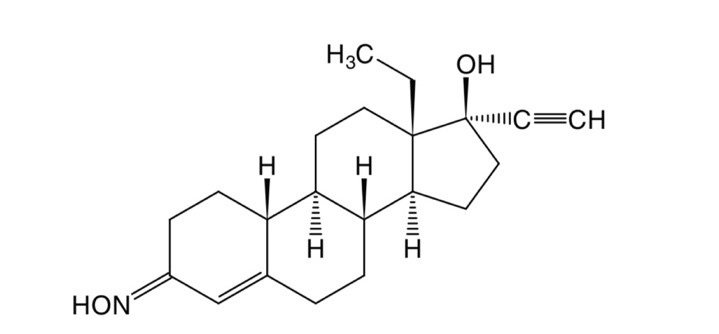
\includegraphics{Images/fig_32.jpg}
    \caption{Norelgestromine (61)}
  \end{figure}
  \item L’étonogestrel : C’est un métabolite dérivé du désogestrel. 
  \begin{figure}[H]
    \centering
    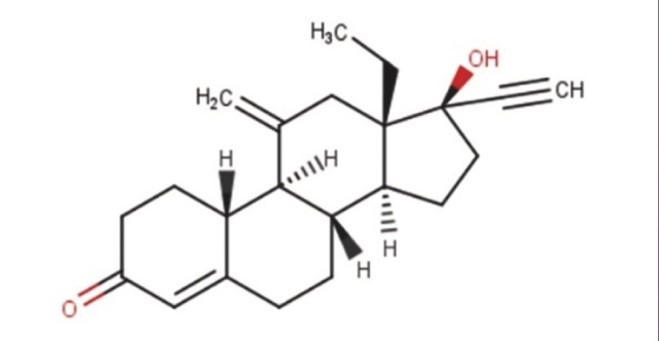
\includegraphics{Images/fig_33.jpg}
    \caption{L’étonogestrel }
  \end{figure}
  \item Le diénogest : C’est un anti-gonadotrope.  
  \begin{figure}[H]
    \centering
    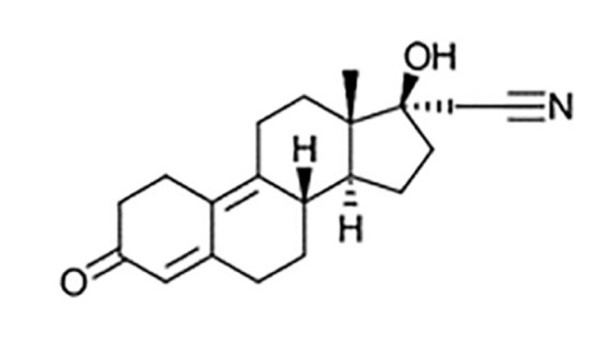
\includegraphics{Images/fig_34.jpg}    
    \caption{Le diénogest (58)}
  \end{figure}

  \item Les dérivés non stéroïdiens de la prégnane comme l’acétate de cyprotérone. (45) 
  \begin{figure}[H]
    \centering
    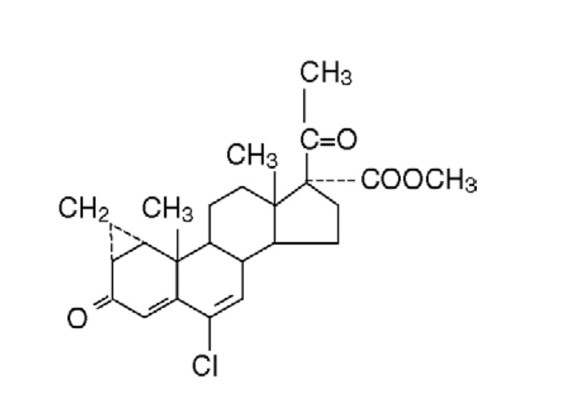
\includegraphics{Images/fig_35.jpg}
    \caption{Acétate de cyprotérone (59)}
    
  \end{figure}
  
\end{itemize}

\noindent \textbf{L’éthinylestradiol} est la forme synthétique de l’hormone œstrogène. Il s’agit de l’œstrogène le plus couramment utilisé dans la contraception. C’est un dérivé du 17$\beta$-estradiol par ajout d’un radical éthinyl en C17. (59) Il a été synthétisé pour la première fois en 1938 et c’est le premier œstrogène actif par voie orale. Il résiste à la dégradation intestinale et hépatique.  

\begin{figure}[H]
  \centering
  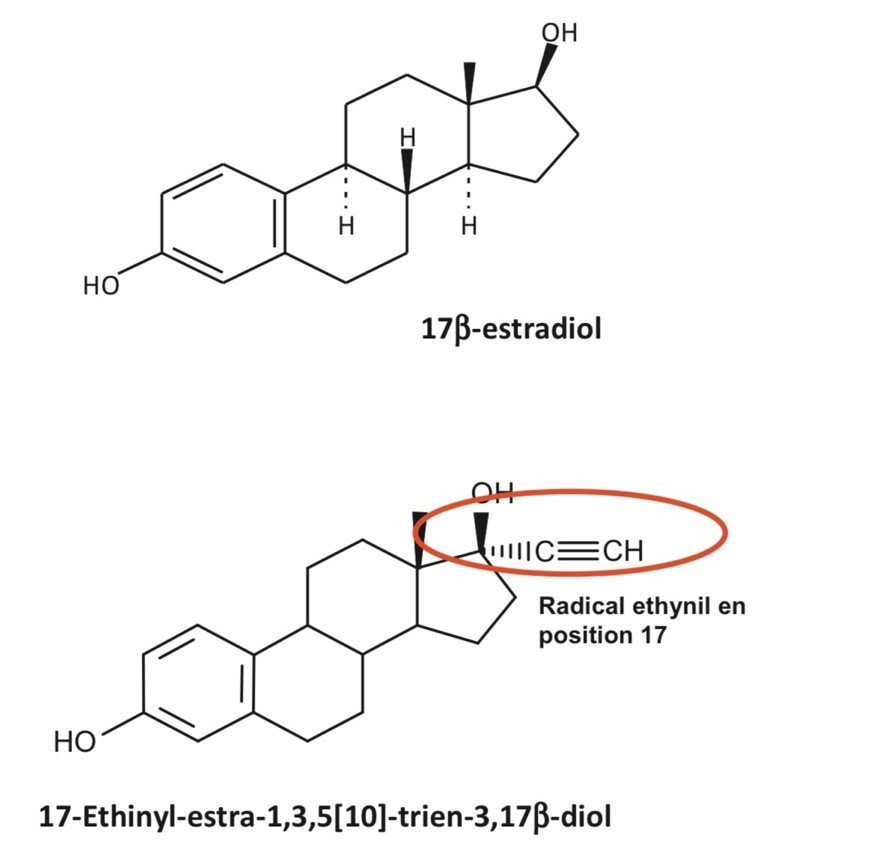
\includegraphics[scale=.6]{Images/fig_36.jpg}
  \caption{17$\beta$-estradiol et éthinylestradiol (62)}
\end{figure}

\noindent Il existe d’autres œstrogènes utilisés pour la contraception, tels que l’œstradiol, le valérate d’œstradiol, etc. (10)

\subsubsection{Les contraceptifs oraux:}

Ils sont aussi connus sous le nom de pilules contraceptives. Ces pilules peuvent être monophasiques, biphasiques ou triphasiques et se présentent en plaquette de 21 pilules ou de 28 pilules. Ce sont des hormones stéroïdiennes. Il en existe deux types, l’un composé uniquement de progestatifs également appelés contraceptifs oraux progestatifs et l’autre d’œstrogènes et de progestatifs également appelés contraceptifs oraux combinés. (2) \\

\noindent Ils sont efficaces avec un taux d’échec compris entre 7,2 et 9\%. Ces médicament sont couramment utilisés dans le cadre d’une contraception réversible et offrent des avantages non contraceptifs tels que: 

\begin{itemize}[label={$\bullet$}, align=right]
  \item	Ils réduisent les risques de certains cancers tels que le cancer de l’ovaire et de l’endomètre,
  \item	Ils régulent le cycle menstruel, aident en cas de règles irrégulières ou abondantes,
  \item Ils traitent les migraines et l’acné causées par les menstruations, 
  \item Ils traitent les troubles dysphoriques prémenstruels, 
  \item Ils aident également à soulager les crampes menstruelles, etc. (63)
\end{itemize}

\subsubsubsection{Les contraceptifs oraux progestatifs:}

Les contraceptifs à progestatifs seul présentent certains avantages: 

\begin{itemize}[label={$\bullet$}, align=right]
  \item	Les femmes qui ne peuvent pas prendre d’œstrogènes pour des raisons de santé ou autres peuvent l’utiliser,
  \item	Le mode de prise est simple,
  \item Le retour à la fertilité est presque immédiat après l’arrêt du traitement,
  \item Les fumeuses de plus de 35 ans peuvent l’utiliser, 
  \item Les femmes qui allaitent peuvent utiliser ce médicament, 
  \item Ils conviennent aux femmes qui souhaitent la dose efficace la plus faible des stéroïdes à des fins contraceptives, etc. (64)
\end{itemize}

\subsubsubsection{Les contraceptifs oraux combinés:}
Ce sont des pilules contraceptives contenant des hormones progestatives et œstrogènes. Leur mécanisme d’action est le suivant: 
\begin{itemize}[label={$\bullet$}, align=right]
  \item	L’inhibition de l’ovulation, empêchant ainsi la libération des ovules par les ovaires. C’est le principal mécanisme d’action. 
  \item Ces pilules épaississent la glaire cervicale, empêchant ainsi les spermatozoïdes de pénétrer. 
  \item	Elles bloquent aussi l’hormone lutéinisante et l’hormone folliculo-stimulante. (65)
\end{itemize}

\noindent Les COC peuvent être classés par générations en fonction de leur compositions (hormones qu’ils contiennent) et de leur évolution dans le temps. Au Maroc, les contraceptifs oraux sont classés en \textbf{quatre générations.}\vspace{2em}


\begin{table}[H]
    \centering
    \renewcommand{\arraystretch}{1.5}
    \begin{spacing}{1.5} % Set line spacing to 1.5
    \begin{tabularx}{\textwidth}{|X|p{8cm}|X|}
        \hline
        \textbf{PREMIERE \newline GENERATION} & \textbf{DOSAGE ETHINYLESTRADIOL \newline DOSAGE PROGESTATIF} & \textbf{TYPES}  \\
        \hline
        Milligynon* & Noréthistérone : 28cp à 0,6mg  &  \\
        \hline
        Triela* & Noréthistérone : 7cp à 0,5mg 
       \begin{itemize}[label={}, nosep]
        \item \hspace{21mm}7cp à 0,75mg
        \item  \hspace{20mm} 7cp à 1mg
    \end{itemize}
Ethinylestradiol : 21cp à 0,035mg 
& Triphasique \\
        \hline
    \end{tabularx}
  \end{spacing}
    \caption{Première génération de contraceptifs oraux au Maroc (66)(4)}
    %\label{tab:my_table}
\end{table}

\begin{table}[H]
  \centering
  \renewcommand{\arraystretch}{1.5}
  \begin{spacing}{1.35} % Set line spacing to 1.5
  \begin{tabularx}{\textwidth}{|X|p{8cm}|X|}
      \hline
      \textbf{DEUXIEME  \newline GENERATION} & \textbf{DOSAGE ETHINYLESTRADIOL \newline DOSAGE PROGESTATIF} & \textbf{TYPES}  \\
      \hline
      Adepal & Lévonorgestrel : 7cp à 0,15 mg
      \begin{itemize}[label={}, nosep]
        \item \hspace{20mm}14cp à 0,20mg 
    \end{itemize} 
    Ethinylestradiol : 21cp à 0,03 mg 
    \begin{itemize}[label={}, nosep]
      \item \hspace{22mm}14cp à 0,04 mg
    \end{itemize}
     & Biphasique \\
      \hline
      Microgynon* & Lévonorgestrel: 21cp à 0,15 mg 
      \newline
      Ethinylestradiol :  21cp à 0,03 mg
& Monophasique \\
\hline
Microval* & Lévonorgestrel : 28cp à 0,03mg 
&  \\  
\hline
Minidril* & Lévonorgestrel : 21cp à 0,15mg  
\newline
Ethinylestradiol : 21cp à 0,03mg 
& Monophasique \\
\hline
Stediril & Norgestrel :         21cp à 0,50mg 
\newline
Ethinylestradiol : 21cp à 0,05mg 
& Monophasique \\
\hline
Trigynon* & Lévonorgestrel : 6cp à 0,05mg  
\begin{itemize}[label={}, nosep]
  \item \hspace{22mm}5cp à 0,075mg 
  \item \hspace{22mm}10cp à 0,125mg 
\end{itemize}

Ethinylestradiol : 6cp à 0,03mg
\begin{itemize}[label={}, nosep]
  \item \hspace{22mm}5cp à 0,04mg 
  \item \hspace{22mm}10cp à 0,03mg  
\end{itemize}
& Triphasique \\
\hline
Trinordiol* & Lévonorgestrel : 6cp à 0,05mg 
\begin{itemize}[label={}, nosep]
  \item \hspace{22mm}5cp à 0,075mg  
  \item \hspace{22mm}10cp à 0,125mg  
\end{itemize} 
Ethinylestradiol : 6cp à 0,03mg
\begin{itemize}[label={}, nosep]
  \item \hspace{22mm}5cp à 0,04mg  
  \item \hspace{22mm}10cp à 0,03mg  
\end{itemize}
\vspace{1em}
& Triphasique \\
      \hline
  \end{tabularx}
\end{spacing}
  \caption{Deuxième génération de contraceptifs oraux au Maroc (66)(4)}
  %\label{tab:my_table}
\end{table}


%%%%%%%%%%%%%%%%%%%%%%%%%%%%%%%%%%%%%%%%5


\begin{table}[H]
  \centering
  \renewcommand{\arraystretch}{1.5}
  \begin{spacing}{1.35} % Set line spacing to 1.5
  \begin{tabularx}{\textwidth}{|X|p{8cm}|X|}
      \hline
      \textbf{TROISIEME   \newline GENERATION} & \textbf{DOSAGE ETHINYLESTRADIOL \newline DOSAGE PROGESTATIF} & \textbf{TYPES}  \\
      \hline
      Cerazette* & Désogestrel : 28cp à 0,075mg
     &  \\
      \hline
      Gracial* & Désogestrel : 7cp à 0,025 mg 
      \begin{itemize}[label={}, nosep]
        \item \hspace{22mm}15cp à 0,125mg
      \end{itemize}
      Ethinylestradiol : 7cp à 0,04mg
      \begin{itemize}[label={}, nosep]
        \item \hspace{22mm}15cp à 0,03mg 
      \end{itemize}
& Combiphasique \\
\hline
Mercilon* & Désogestrel : 21cp à 0,15 mg 
\newline
Ethinylestradiol : 21cp à 0,02mg
& Monophasique \\  
\hline
Microdiol* & Désogestrel : 21cp à 0,15 mg   
\newline
Ethinylestradiol : 21cp à 0,03mg  
& Monophasique \\
\hline
Minulet* &Gestodène : 21cp à 0,75mg  
\newline
Ethinylestradiol : 21cp à 0,03mg  
& Monophasique \\
\hline
Moneva* & Gestodène : 21cp à 0,75mg   
\newline
Ethinylestradiol : 21cp à 0,03mg 
& Monophasique \\
\hline
Phaeva* & Gestodène : 6cp à 0,05mg 
\begin{itemize}[label={}, nosep]
  \item \hspace{22mm}5cp à 0,07mg  
  \item \hspace{22mm}10cp à 0,07mg  
\end{itemize} 
Ethinylestradiol : 6cp à 0,03mg
\begin{itemize}[label={}, nosep]
  \item \hspace{22mm}5cp à 0,04mg   
  \item \hspace{22mm}10cp à 0,03mg   
\end{itemize}
\vspace{1em}
& Triphasique \\
      \hline
  \end{tabularx}
\end{spacing}
  \caption{Troisième génération de contraceptifs oraux au Maroc (66)(4)}
  %\label{tab:my_table}
\end{table}


\begin{table}[H]
  \centering
  \renewcommand{\arraystretch}{1.5}
  \begin{spacing}{1.5} % Set line spacing to 1.5
  \begin{tabularx}{\textwidth}{|X|p{8cm}|X|}
      \hline
      \textbf{QUATRIEME GENERATION} &  \\
      \hline
       
      Jasmine* & Drospirénone \newline Ethinylestradiol
       \\
      \hline
      Yaz* & Drospirénone \newline Ethinylestradiol
      \\
      \hline
  \end{tabularx}
\end{spacing}
  \caption{Quatrième génération de contraceptifs oraux au Maroc (66)}
  %\label{tab:my_table}
\end{table}

\noindent Bien que les COC soient généralement sûrs pour les femmes en bonne santé a faible dose, ils peuvent s’avérer dangereux pour les femmes présentant des facteurs de risques. (67)\\

\noindent \textbf{Les effets bénéfiques des COC sont présentés ci-dessous:}

\begin{table}[H]
  \centering
  \begin{tabular}{c}
      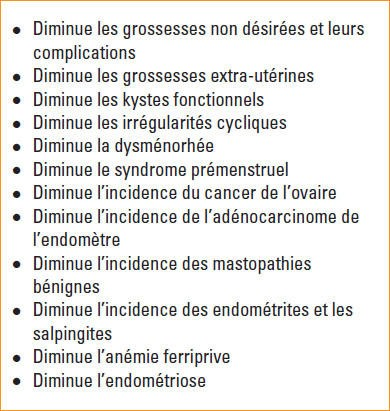
\includegraphics[scale=3.5]{Images/tab_6.jpg} \\
  \end{tabular}
  \caption{Principaux effets bénéfiques des contraceptifs oraux combinés (68)}
  % \label{tab:contra_indications}
\end{table}

\textbf{Les contre-indications des COC sont présentées ci-dessous :}

\begin{table}[H]
\centering
\begin{tabular}{c}
    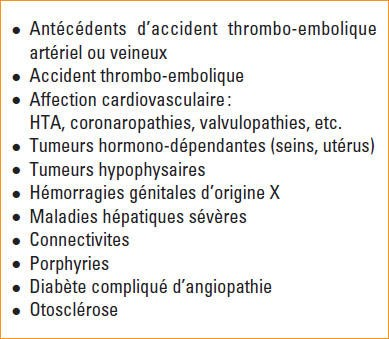
\includegraphics[scale=4.2]{Images/tab_7.jpg} \\
\end{tabular}
\caption{Contre-indications absolues des contraceptifs oraux combinés (68)}
% \label{tab:contra_indications}
\end{table}

\subsubsection{Les contraceptifs injectables:}

Les contraceptifs injectables sont des contraceptifs hormonaux administrés par voie intramusculaire (4) ou sous cutanée. Leur efficacité a été prouvée et ils sont utilisés dans de nombreux pays. Il en existe maintenant qui peuvent être auto-administrés. (69) \\

\noindent Les contraceptifs injectable peuvent être classés en deux catégories : les contraceptifs injectables à progestatif seul et les contraceptifs injectables combinés. \\

\hspace{1em}\textbf{•	Les contraceptifs injectables à progestatif seul : }\vspace*{1em}

\begin{figure}[H]
  \centering	
  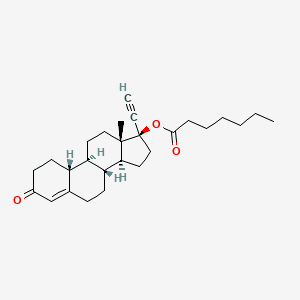
\includegraphics{Images/fig_37.jpg}
  \caption{Énanthate de noréthistérone (70)}
  
\end{figure}

\begin{figure}[H]
  \centering
  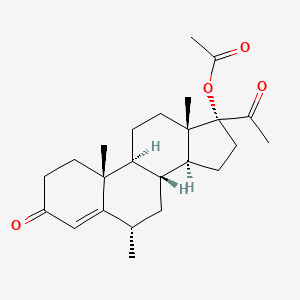
\includegraphics{Images/fig_38.png}
  \caption{Acétate de médroxyprogestérone (71)}  
\end{figure}


\begin{figure}[H]
  \centering
  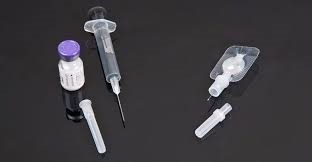
\includegraphics{Images/fig_39.jpg}
  \caption{A gauche, DMPA-IM et à droite DMPA-SC (72)}
  
\end{figure}

\hspace{1em}\textbf{•	Les contraceptives injectables combinés : }\vspace*{1em}

\noindent ls contiennent de la progestérone et des œstrogènes. Ils sont administrés tous les mois. (73)

\subsubsection{Les implants sous cutanés: }
L’implant est un petit bâtonnet en plastique, inséré sous la peau à la face interne du bras, au-dessus du coude qui libère une faible dose régulière de l’hormone progestative. Il est utilisé pour la contraception à long terme car il peut assurer une couverture contraceptive pendant 3 à 5 ans. (74) \\
\noindent Le premier contraceptif implantable est le norplant* lévonorgestrel (LNG). (75) Il contenait 216mg de LNG, mais il n’est plus commercialisé. Les implants actuellement disponibles sont Implanon* etonogestrel 68mg, Jadelle* LNG 150mg, etc. Leur mécanisme d’action est l’épaississement de la glaire cervicale pour empêcher la pénétration des spermatozoïdes et l’inhibition de l’ovulation. (76)\\

\noindent Ils constituent une méthode de contraception très efficace. En plus d’être très efficaces, ils présentent certains avantages : 
\begin{itemize}
  \item Ils sont réversibles,
  \item Ils constituent une contraception de longue durée, 
  \item	L’efficacité de cette méthode ne dépend pas de l’utilisatrice
  \item Ils peuvent être utilisés par certaines personnes souffrant de complications médicales en l’absence de contre-indications. (77) 
\end{itemize}

\noindent Ces implants ont des effets indésirables tels que : 

\begin{itemize}
  \item La prise de poids, 
  \item Les troubles menstruels tels que l’aménorrhée, le spotting et les métrorragies,
  \item	Les troubles menstruels tels que l’aménorrhée, le spotting et les métrorragies,
  \item	La céphalée, 
  \item	La mastodynie, 
  \item	L’acné, etc. (78)
\end{itemize}

\begin{figure}[H]
  \centering
  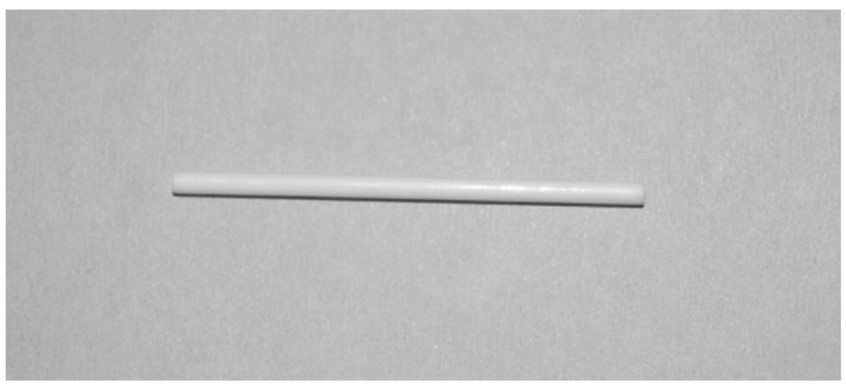
\includegraphics[scale=1.2]{Images/fig_40.jpg}
  \caption{Implant sous cutané (46)}
    
\end{figure}

\subsubsection{Les contraceptifs d’urgence : }
Ils interviennent après un rapport sexuel non ou mal protégé pour éviter une grossesse. (79) Ils sont plus efficaces s’ils sont utilisés tôt. (80) In en existe deux types : les pilules contraceptives d’urgence et le stérilet en cuivre. (81)

\subsubsubsection{Les pilules hormonales contraceptives d’urgence : }
Elles sont également appelées pilules du lendemain et doivent être utilisées dans les 5 jours suivant le rapport sexuel non protégé. (80) Ces pilules ne sont pas des pilules abortives et ne peuvent pas être utilisées pour interrompre une grossesse déjà établie. Le mécanisme d’action de ces pilules est de retarder ou empêcher l’ovulation. Elles ne sont pas efficaces après l’ovulation. (82) Elles comprennent la pilule progestative contenant du LNG, la pilule anti progestative contenant de l’acétate d’ulipristal et la pilule contraceptive d’urgence combinée. Elles sont efficaces, mais certains facteurs peuvent affecter leur efficacité: 

\begin{itemize}
  \item	Les interactions médicamenteuses,
  \item	Le poids de l’utilisatrice,
  \item Le moment du rapport sexuel non protégé et de l’administration du contraceptif de la pilule, cette dernière étant plus efficace lorsqu’elle est administrée tôt,
  \item	L’ovulation : L’efficacité de la pilule diminue si elle est prise le jour de l’ovulation,
  \item	D’autres rapports sexuels non protégés après la prise de la pilule,  
  \item La malabsorption ou les vomissements. (81) 
\end{itemize}

\noindent Ces pilules ne nécessitent pas d’ordonnance, mais il est important de demander l’avis d’un professionnel de la santé avant de les utiliser. Elles empêchent l’ovulation, la fécondation ou l’implantation de l’ovule fécondé. Elles ne doivent pas être utilisées de manière systématique, mais uniquement en cas d’urgence, par exemple : 

\begin{itemize}
  \item En cas d’oubli de pilules contraceptives orales, 
  \item En cas de retard de réinjection des contraceptifs injectables, 
  \item En cas de déchirure ou de glissement du préservatif,
  \item En cas d’expulsion d’un stérilet. (83)
\end{itemize}

\vspace*{1em}

\noindent\textbf{Les avantages de la contraception d’urgences sont: }

\begin{itemize}
  \item Elle ne présente d’effets indésirables à long terme,
  \item Son taux d’échec est faible, 
  \item Elle peut être obtenue facilement de santé, 
  \item	Elle peut être prise jusqu’à 72 heures après un rapport sexuel non protégé,
  \item	La pilule est facile à prendre, 
  \item Elle présente moins d’effets secondaires par rapport à d’autres contraceptifs hormonaux combinés. 
\end{itemize}

\vspace*{1em}

\noindent\textbf{Les inconvénients de la contraception d’urgence sont: }

\begin{itemize}
  \item	Elle peut perturber le cycle menstruel, 
  \item Elle est inefficace si elle est prise après 72 à 120 heures après un rapport sexuel non protégé, 
  \item Elle ne protège pas contre les infections sexuellement transmissibles,
  \item Elle peut provoquer des nausées et des vomissements. (84)
\end{itemize}

\subsubsubsection{Les dispositifs intra-utérins: }
Le stérilet en cuivre a un effet contraceptif d’urgence s’il est utilisé dans les 5 à 7 jours suivant un rapport sexuel non protégé. (80) Ce sont les contraceptives d’urgences les plus efficaces, avec un taux de réussite de plus de 99\%. Ils peuvent être utilisés même après l’ovulation. Les ions Cu2+ affectent la fonction des spermatozoïdes et empêchent ainsi la fécondation. (81) 

\subsubsection{Le patch contraceptif: }

Ce contraceptif hormonal se porte sur la peau. Il s’agit d’un contraceptif hormonal combiné contenant de la progestérone et de l’œstrogène qui sont libérés dans le sang à travers la peau. Il est changé chaque semaine pendant trois semaines, puis une semaine de repos est observée. Il s’agit d’une méthode de contraception efficace. (85)   

\begin{figure}[H]
  \centering
  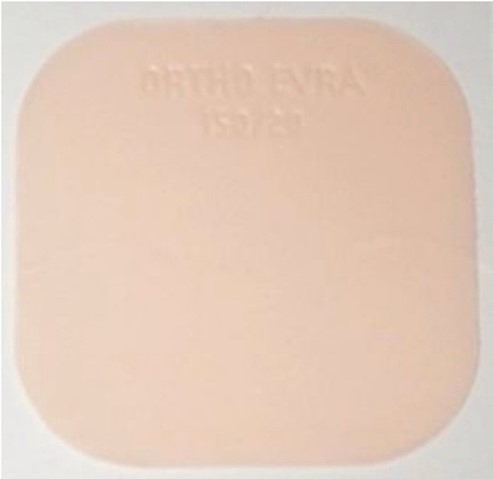
\includegraphics{Images/fig_41.jpg}
  \caption{Patch contraceptif (86)} 
\end{figure}

\subsubsection{L’anneau vaginal: }
Il s’agit d’un dispositif contraceptif contenant des hormones contraceptives qui sont libérées pour empêcher la grossesse en inhibant l’ovulation. Il contient une combinaison de progestérone et d’œstrogène. Il est utilisé pendant une période de trois semaines, puis retiré pour une pause d’une semaine. Il constitue une méthode de contraception très efficace. Il présente certains avantages non contraceptifs, notamment: 

\begin{itemize}
  \item	Il permet de traiter le syndrome des ovaires polykystiques, 
  \item Il est utilisé pour traiter l’endométriose, 
  \item	Il permet de traiter la dysménorrhée, 
  \item	Il permet de traiter la dysménorrhée, 
  \item	Il constitue une méthode contraceptive réversible qui permet un retour quasi immédiat à la fertilité, 
  \item	Il réduit les crampes menstruelles, 
  \item	Il aide à réguler le cycle menstruel. (87) 
\end{itemize}

\begin{figure}[H]
  \centering
  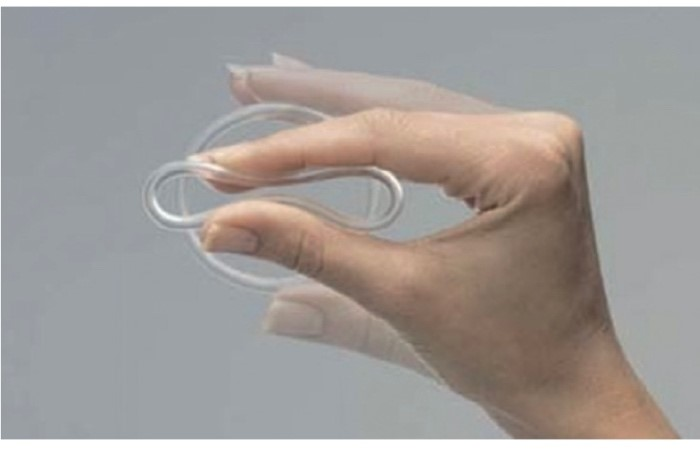
\includegraphics[scale=1.1]{Images/fig_42.jpg}
  \caption{Anneau vaginal (45)}
  
\end{figure}

\subsection{Les méthodes chirurgicales : }

Ces méthodes de contraception sont principalement utilisées par les personnes qui ne veulent plus avoir d’enfants pour des raisons médicales ou autres.

\subsubsection{La ligature des trompes de Fallope: }

La ligature des trompes de Fallope, également connue sous le nom de stérilisation féminine, est un moyen de contraception permanent pour les femmes. Elle consiste à bloquer les trompes de Fallope afin d’empêcher les ovules d’atteindre l’utérus et d’être fécondés par les spermatozoïdes. \vspace{1em}

\noindent Parmi les méthodes de stérilisation féminine, on peut citer l’interruption des trompes de Fallope par laparoscopie, la salpingectomie par laparoscopie, la stérilisation par hystéroscopie, etc. (88)

\begin{figure}[H]
  \centering
  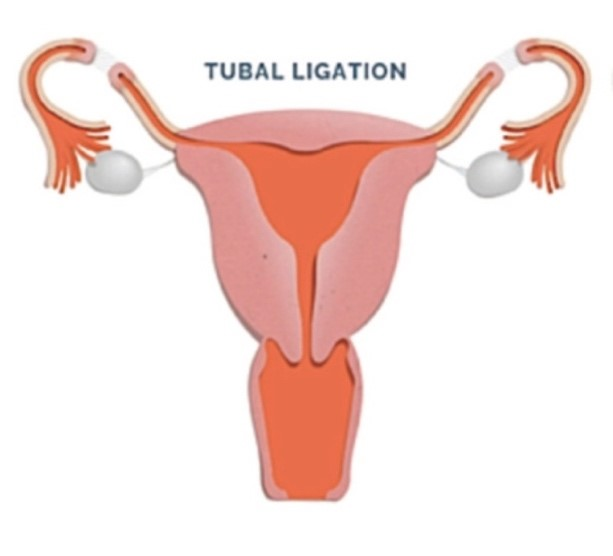
\includegraphics{Images/fig_43.jpg}
  \caption{La ligature tubaire (89)}
\end{figure}

\subsubsection{La vasectomie: }

\noindent La vasectomie et les préservatifs sont les moyens de contraception masculine disponibles. (90) Le retrait, qui est une méthode contraceptive naturelle, peut également être utilisé, mais il est moins efficace. (91)\\

\noindent La vasectomie est une méthode de contraception permanente pour les hommes. Elle consiste à couper ou à ligaturer les canaux déférents qui achemine les spermatozoïdes du testicule à l’urèthre. Elle est très efficace. (92) Son taux d’échec est inférieur à 0,014\%. (91) Il s’agit d’une intervention chirurgicale simple, pratiquée par des urologues. \\

\noindent Les techniques de vasectomie sont les différentes méthodes qui peuvent être utilisées pour effectuer une vasectomie,  telles que la technique d’incision conventionnelle, la vasectomie sans bistouri et la vasectomie modifiée sans bistouri. Les méthodes d’occlusion vasale, c’est-à-dire les méthodes utilisées pour bloquer les canaux déférents, sont l’excision et la ligature, la cautérisation, l’interposition fasciale, la cautérisation plus l’interposition fasciale et la vasectomie ouverte. (93)

\begin{figure}[H]
  \centering
  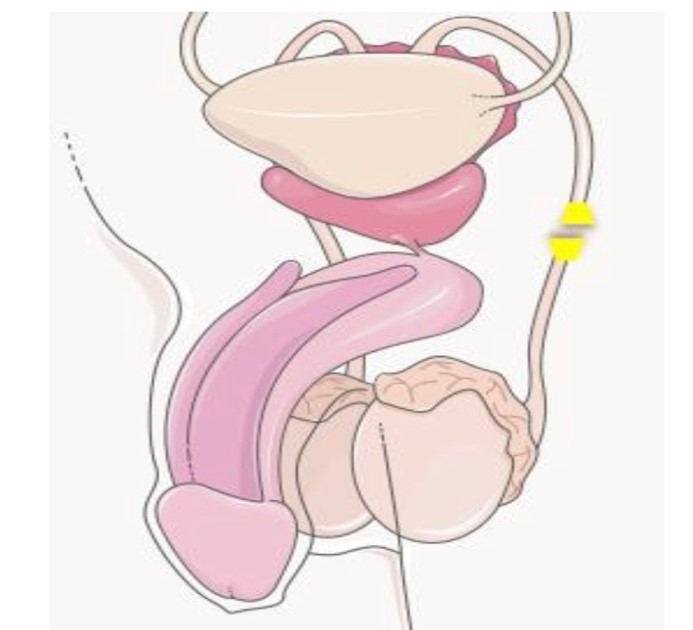
\includegraphics{Images/fig_44.jpg}
  \caption{La vasectomie (28)}
  
\end{figure}

\section{Les particularités des contraceptifs injectables }

\noindent Les contraceptifs injectables constituent une option de contraception hormonale, pouvant être administrée soit par voie intramusculaire ou sous-cutanée. Voici quelques-unes de leur particularités :  


\subsection{Les différents types: }

Les types de contraceptifs injectables disponibles au Maroc sont le Depoprovera* (acétate de dépo-médroxy-progestérone) et le Noristerat* ou Megestron*(énantate de noréthistérone). (4) Le Depoprovera* est administré tous les trois mois et le Noristerat* tous les deux mois. 

\subsection{Composition: }

Les contraceptifs injectables progestatifs sont composés uniquement de progestérone, tandis que les contraceptifs injectables combinés sont composés de progestérone et d’œstrogène. 


\begin{table}[H]
  \centering
  \renewcommand{\arraystretch}{1.5}
  \begin{spacing}{1.5} % Set line spacing to 1.5
  \begin{tabularx}{\textwidth}{|X|p{3cm}|X|X|p{3.3cm}|X|}
      \hline
      \textbf{Principe actif} & \textbf{Nom\newline commercial} & \textbf{Charge}  & \textbf{Volume}  & \textbf{Voie d’administration} & \textbf{Durée}\\
      \hline
      DMPA & Depo-Provera*  & 150 mg & 1 mL & Intra musculaire & 3 mois\\
      \hline
      DMPA & Depo SubQ Provera 104*, Sayana*, Sayana Press*  & 104 mg & 0,65 mL & Sous cutanée  & 3 mois\\
      \hline
      NET-EN & Noristerat* & 200 mg  & 1 mL & Intra musculaire & 2 mois\\
      \hline
  \end{tabularx}
\end{spacing}
  \caption{Les différents types de contraceptifs injectables progestatifs (19)}
  %\label{tab:my_table}
\end{table}

\textbf{Les contraceptifs injectables combinés} sont administrés mensuellement par voie intramusculaire. Ils ne sont pas couramment utilisés mais les contraceptifs disponibles sont présentés dans le tableau ci-dessous : 

\begin{table}[H]
  \centering
  \renewcommand{\arraystretch}{1.5}
  \begin{spacing}{1.5} % Set line spacing to 1.5
  \begin{tabularx}{\textwidth}{|X|X|X|}
      \hline
      \textbf{Progestin } & \textbf{Estrogen} & \textbf{Nom commercial} \\
      \hline
      AMPR 25mg & Cypionate d’estradiol 5mg  & Cyclofem*\\
      \hline
      NET-EN 50mg  & Valérate d’estradiol 5mg  &  Mesigyna*\\
      \hline
      Acétophénide  \hspace{2cm} de dihyroxyprogestérone 150mg & Enanthate d’estradiol 10mg  & Deladroxate* \\
      \hline
  \end{tabularx}
\end{spacing}
  \caption{Les différents types de contraceptifs injectables combinés (94)}
  %\label{tab:my_table}
\end{table}

\subsection{Mécanisme d’action: }

Les contraceptifs injectables ont pour principal mécanisme d’action, l’inhibition de l’ovulation. (95) Cela se fait par la suppression de l’axe hypothalamique/pituaire/ovarien. (96) Les deux contraceptifs injectables disponibles au Maroc, le DMPA et le NET-EN, ont pratiquement les mêmes mécanismes d’action qui sont :  

\begin{itemize}
  \item La suppression de l’hormone folliculostimulante et de l’hormone lutéinisante pour inhiber l’ovulation 
  \item Empêcher le mouvement des spermatozoïdes dans la cavité utérine en augmentant la viscosité de la glaire cervicale
  \item Empêcher la nidation en amincissant la muqueuse endométriale. (97) 
\end{itemize}

\subsection{3.4. Indications:}

Les contraceptifs injectables progestatifs et les contraceptifs injectables combinés sont tous les deux utilisés pour la contraception de longue durée. La durée peut être d’un, deux ou trois mois selon le type de contraceptif injectable utilisé. 

\subsection{Contre-indications:}

Les contraceptifs injectables présentent certaines contre-indications : 

\begin{itemize}
  \item  Ils ne doivent pas être utilisés en cas d’hypersensibilité à l’un des composants du contraceptif,
  \item Ils ne doivent pas être utilisés en cas de saignements vaginaux non diagnostiqués, 
  \item Ils ne doivent pas être utilisés chez les femmes atteintes d’un cancer du sein,
  \item Ils ne doivent pas être utilisé pendant la grossesse. (98)
\end{itemize}

\subsection{Interactions médicamenteuses: }

Les interactions médicamenteuses peuvent être soit pharmacodynamiques, c’est-à-dire que deux médicaments ou plus interagissent et produisent des effets synergiques ou antagonistes, soit pharmacocinétiques, c’est-à-dire que l’absorption, la distribution, le métabolisme ou l’élimination d’un médicament est modifié en raison de son interaction avec d’autres médicaments, réduisant ou augmentant ainsi son effet. Ces interactions médicamenteuses peuvent altérer la sécurité et l’efficacité de médicaments. \\

\noindent Quelques interactions médicamenteuses avec les contraceptifs injectables sont les suivantes : 

\begin{itemize}[label={$\Rightarrow$}, align=right]
  \item Les inducteurs enzymatiques, qui réduisent l’effet des contraceptifs : 
  \begin{itemize}[label={$\bullet$}, nosep]
    \item Les anticonvulsivants comme la phénytoïne, la carbamazépine, le phénobarbital, etc., sont déconseillés, tandis que le rufinamide est doit être utilisé avec précaution,
    \item Les antidépresseurs comme le millepertuis sont contre-indiqués, 
    \item Les antifongiques comme la griséofulvine doit être utilisés avec précaution,
    \item Les antibiotiques comme la rifabutine et la rifampicine sont déconseillés, 
    \item Les antirétroviraux tels que l’efavirenz et l’elfitégravir, etc., doivent être utilisés avec précaution, lotanavir + ritonavir, atazanivir + ritonavir, saquinavir + ritonavir, etc., sont déconseillés
    \item Le modanafil est également déconseillé,
    \item L’aprépitant et le bosétan doivent être utilisés avec précaution. 
  \end{itemize}

  \item Les inhibiteurs enzymatiques :
  \begin{itemize}[label={$\bullet$}, nosep]    
    \item Les antifongiques azolés comme le voriconazole, le kétoconazole etc., 
    \item Les antiinflammatoires non stéroïdiens comme l’étoricoxib, 
    \item Le bocéprévir, 
    \item L’atorvastatine. (99)
  \end{itemize}
\end{itemize}


\subsection{Effets indésirables: }

Les effets indésirables des contraceptifs injectables progestatifs sont les suivants: 

\begin{itemize}[label={$\bullet$}, nosep] 
  \item Ils peuvent retarder le retour de la fertilité, 
  \item Ils peuvent provoquer des saignements irréguliers,
  \item Ils peuvent être à l’origine de changements d’humeur, voire d’une dépression. 
\end{itemize}

\vspace{1em}

\noindent Les effets indésirables communs aux contraceptifs injectables progestatifs et aux contraceptifs injectables combinés sont les suivants : 

\begin{itemize}
  \item	Ils peuvent provoquer des maux de tête, 
  \item	Ils peuvent entraîner la prise de poids, 
  \item	Ils peuvent aussi provoquer des douleurs osseuses, 
  \item	Ils peuvent provoquer une sensibilité des seins, 
  \item	Ils peuvent également causer l’aménorrhée, le spotting et la sécheresse vaginale. (100)
\end{itemize}

\subsection{Avantages et inconvénients}

\subsubsection{Avantages: }
Les contraceptifs injectables présentent généralement les avantages suivants : 

\begin{itemize}
  \item Ils permettent une contraception de longue durée, 
  \item Leur utilisation est facile,
  \item Ils sont efficaces avec un taux d’échec très faible, 
  \item Ils constituent une méthode de contraception temporaire,   
  \item	Ce moyen de contraception ne perturbe pas les rapports sexuels. 
\end{itemize}

\noindent Les avantages des contraceptifs injectables progestatifs sont les suivants : 

\begin{itemize}
  \item	Les femmes allaitantes peuvent les utiliser 6 semaines après l’accouchement, 
  \item	Les fumeuses peuvent y recourir, 
  \item	Ils ne sont pas limités à certains âges, 
  \item	Ils ne présentent pas d’effets indésirables liés à l’œstrogène, 
  \item	Les femmes souffrant de certaines maladies comme la cardiopathie valvulaire, la drépanocytose, la tuberculose, l’épilepsie, les maladies thyroïdiennes, etc., peuvent les utiliser comme moyen de contraception. (94)       
\end{itemize}

\subsubsection{Inconvénients: }

Les inconvénient des contraceptifs injectables sont les suivants: 

\begin{itemize}
  \item	Ils sont irréversibles dans la durée prescrite, 
  \item Leur effet peut durer jusqu’à 12 mois après l’injection,
  \item Leur couverture contraceptive est plus courte que celle des autres contraceptifs à long terme, 
  \item	Douleur au site d’injection. (19)
\end{itemize}

\subsection{Pharmacocinétiques :}

Le DMPA est une suspension aqueuse cristalline de 17-acétoxy-6-méthylprogestérone. Dans les 30 minutes qui suivent son injection intramusculaire, il se retrouve dans la circulation systémique et atteint son niveau d’effet contraceptif dans les 24heures. Sa concentration est maximale au cours des trois premières semaines suivant l’injection et diminue après 90 à 190 jours. Le NET-EN, quant à lui, sa concentration diminue dans les 80 à 110 jours suivant l’injection, tandis que pour le Mesigyna* et Cyclofem*, elle diminue au bout de 14 jours. (94)

\subsection{Efficacité: }

la contraception injectable est un moyen de contraception très efficace. Le DMPA, qui est un contraceptif de 3 mois, a un effet qui peut durer jusqu’à 4 mois. Ces contraceptifs ont un taux d’échec très faible. Selon certains essais cliniques, le DMPA a un taux d’échec d 0,1\% à 12 mois et de 0,4\% à 24 mois, le NET-EN, de 0,4\% à 12 mois et 0,6\% à 24 mois, le Mesigyna de 0,4\% à 12 mois et le Lunelle de 0,2\% à 12 mois. (94) 

\pagebreak


